% Created by tikzDevice version 0.7.0 on 2014-06-30 20:14:08
% !TEX encoding = UTF-8 Unicode
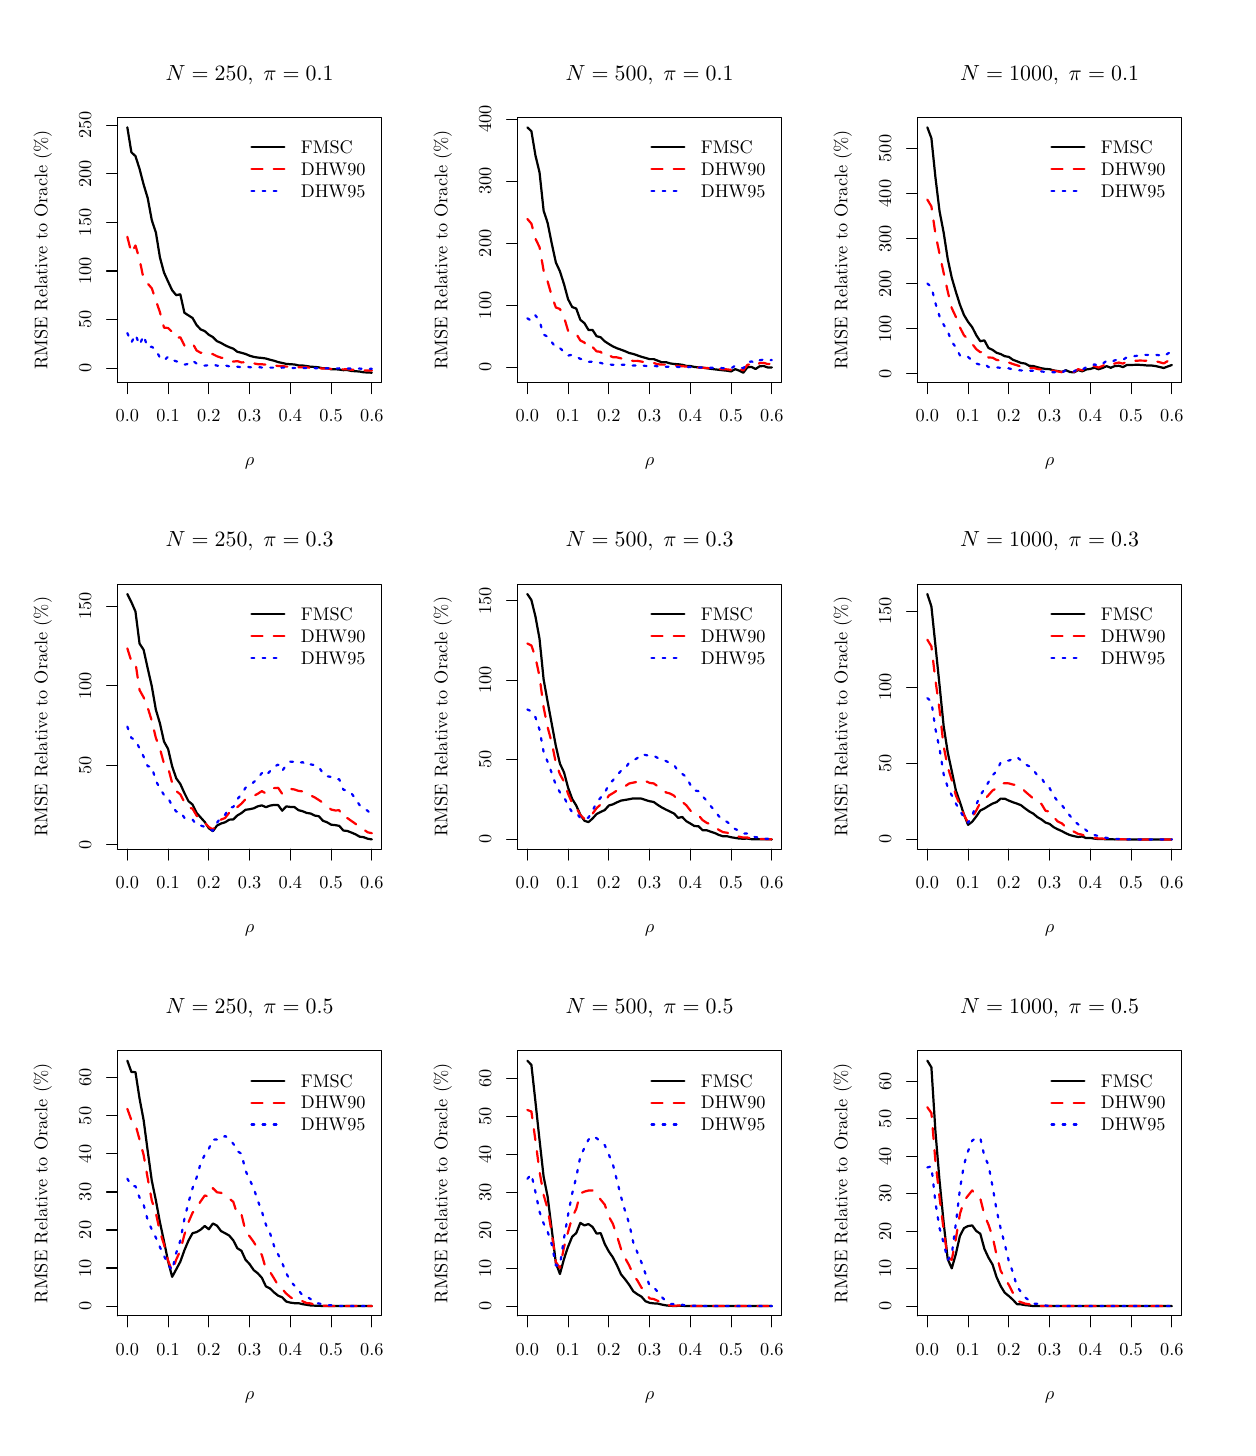
\begin{tikzpicture}[x=1pt,y=1pt]
\definecolor[named]{fillColor}{rgb}{1.00,1.00,1.00}
\path[use as bounding box,fill=fillColor,fill opacity=0.00] (0,0) rectangle (433.62,505.89);
\begin{scope}
\path[clip] ( 32.47,377.65) rectangle (127.91,473.42);
\definecolor[named]{drawColor}{rgb}{0.00,0.00,0.00}

\path[draw=drawColor,line width= 0.8pt,line join=round,line cap=round] ( 36.01,469.87) --
	( 37.48,460.84) --
	( 38.95,459.47) --
	( 40.42,454.88) --
	( 41.90,449.20) --
	( 43.37,444.31) --
	( 44.84,436.37) --
	( 46.32,431.92) --
	( 47.79,422.88) --
	( 49.26,417.40) --
	( 50.73,414.15) --
	( 52.21,410.98) --
	( 53.68,409.22) --
	( 55.15,409.55) --
	( 56.63,402.87) --
	( 58.10,401.92) --
	( 59.57,400.98) --
	( 61.04,398.42) --
	( 62.52,396.84) --
	( 63.99,396.24) --
	( 65.46,394.91) --
	( 66.93,394.07) --
	( 68.41,392.60) --
	( 69.88,391.96) --
	( 71.35,391.11) --
	( 72.83,390.43) --
	( 74.30,389.89) --
	( 75.77,388.76) --
	( 77.24,388.40) --
	( 78.72,387.98) --
	( 80.19,387.35) --
	( 81.66,386.93) --
	( 83.14,386.68) --
	( 84.61,386.55) --
	( 86.08,386.34) --
	( 87.55,385.90) --
	( 89.03,385.53) --
	( 90.50,385.04) --
	( 91.97,384.74) --
	( 93.44,384.39) --
	( 94.92,384.27) --
	( 96.39,384.19) --
	( 97.86,383.85) --
	( 99.34,383.80) --
	(100.81,383.61) --
	(102.28,383.36) --
	(103.75,383.30) --
	(105.23,383.13) --
	(106.70,382.78) --
	(108.17,382.87) --
	(109.65,382.43) --
	(111.12,382.47) --
	(112.59,382.33) --
	(114.06,382.13) --
	(115.54,382.16) --
	(117.01,381.82) --
	(118.48,381.74) --
	(119.95,381.63) --
	(121.43,381.34) --
	(122.90,381.30) --
	(124.37,381.20);
\end{scope}
\begin{scope}
\path[clip] (  0.00,  0.00) rectangle (433.62,505.89);
\definecolor[named]{drawColor}{rgb}{0.00,0.00,0.00}

\path[draw=drawColor,line width= 0.4pt,line join=round,line cap=round] ( 36.01,377.65) -- (124.37,377.65);

\path[draw=drawColor,line width= 0.4pt,line join=round,line cap=round] ( 36.01,377.65) -- ( 36.01,373.69);

\path[draw=drawColor,line width= 0.4pt,line join=round,line cap=round] ( 50.73,377.65) -- ( 50.73,373.69);

\path[draw=drawColor,line width= 0.4pt,line join=round,line cap=round] ( 65.46,377.65) -- ( 65.46,373.69);

\path[draw=drawColor,line width= 0.4pt,line join=round,line cap=round] ( 80.19,377.65) -- ( 80.19,373.69);

\path[draw=drawColor,line width= 0.4pt,line join=round,line cap=round] ( 94.92,377.65) -- ( 94.92,373.69);

\path[draw=drawColor,line width= 0.4pt,line join=round,line cap=round] (109.65,377.65) -- (109.65,373.69);

\path[draw=drawColor,line width= 0.4pt,line join=round,line cap=round] (124.37,377.65) -- (124.37,373.69);

\node[text=drawColor,anchor=base,inner sep=0pt, outer sep=0pt, scale=  0.66] at ( 36.01,363.40) {0.0};

\node[text=drawColor,anchor=base,inner sep=0pt, outer sep=0pt, scale=  0.66] at ( 50.73,363.40) {0.1};

\node[text=drawColor,anchor=base,inner sep=0pt, outer sep=0pt, scale=  0.66] at ( 65.46,363.40) {0.2};

\node[text=drawColor,anchor=base,inner sep=0pt, outer sep=0pt, scale=  0.66] at ( 80.19,363.40) {0.3};

\node[text=drawColor,anchor=base,inner sep=0pt, outer sep=0pt, scale=  0.66] at ( 94.92,363.40) {0.4};

\node[text=drawColor,anchor=base,inner sep=0pt, outer sep=0pt, scale=  0.66] at (109.65,363.40) {0.5};

\node[text=drawColor,anchor=base,inner sep=0pt, outer sep=0pt, scale=  0.66] at (124.37,363.40) {0.6};

\path[draw=drawColor,line width= 0.4pt,line join=round,line cap=round] ( 32.47,382.86) -- ( 32.47,470.65);

\path[draw=drawColor,line width= 0.4pt,line join=round,line cap=round] ( 32.47,382.86) -- ( 28.51,382.86);

\path[draw=drawColor,line width= 0.4pt,line join=round,line cap=round] ( 32.47,400.42) -- ( 28.51,400.42);

\path[draw=drawColor,line width= 0.4pt,line join=round,line cap=round] ( 32.47,417.97) -- ( 28.51,417.97);

\path[draw=drawColor,line width= 0.4pt,line join=round,line cap=round] ( 32.47,435.53) -- ( 28.51,435.53);

\path[draw=drawColor,line width= 0.4pt,line join=round,line cap=round] ( 32.47,453.09) -- ( 28.51,453.09);

\path[draw=drawColor,line width= 0.4pt,line join=round,line cap=round] ( 32.47,470.65) -- ( 28.51,470.65);

\node[text=drawColor,rotate= 90.00,anchor=base,inner sep=0pt, outer sep=0pt, scale=  0.66] at ( 22.97,382.86) {0};

\node[text=drawColor,rotate= 90.00,anchor=base,inner sep=0pt, outer sep=0pt, scale=  0.66] at ( 22.97,400.42) {50};

\node[text=drawColor,rotate= 90.00,anchor=base,inner sep=0pt, outer sep=0pt, scale=  0.66] at ( 22.97,417.97) {100};

\node[text=drawColor,rotate= 90.00,anchor=base,inner sep=0pt, outer sep=0pt, scale=  0.66] at ( 22.97,435.53) {150};

\node[text=drawColor,rotate= 90.00,anchor=base,inner sep=0pt, outer sep=0pt, scale=  0.66] at ( 22.97,453.09) {200};

\node[text=drawColor,rotate= 90.00,anchor=base,inner sep=0pt, outer sep=0pt, scale=  0.66] at ( 22.97,470.65) {250};

\path[draw=drawColor,line width= 0.4pt,line join=round,line cap=round] ( 32.47,377.65) --
	(127.91,377.65) --
	(127.91,473.42) --
	( 32.47,473.42) --
	( 32.47,377.65);
\end{scope}
\begin{scope}
\path[clip] (  0.00,337.26) rectangle (144.54,505.89);
\definecolor[named]{drawColor}{rgb}{0.00,0.00,0.00}

\node[text=drawColor,anchor=base,inner sep=0pt, outer sep=0pt, scale=  0.79] at ( 80.19,486.92) {\bfseries $N=250, \;\pi=0.1$};

\node[text=drawColor,anchor=base,inner sep=0pt, outer sep=0pt, scale=  0.66] at ( 80.19,347.56) {$\rho$};

\node[text=drawColor,rotate= 90.00,anchor=base,inner sep=0pt, outer sep=0pt, scale=  0.66] at (  7.13,425.53) {RMSE Relative to Oracle (\%)};
\end{scope}
\begin{scope}
\path[clip] ( 32.47,377.65) rectangle (127.91,473.42);
\definecolor[named]{drawColor}{rgb}{1.00,0.00,0.00}

\path[draw=drawColor,line width= 0.8pt,dash pattern=on 4pt off 4pt ,line join=round,line cap=round] ( 36.01,430.32) --
	( 37.48,424.49) --
	( 38.95,427.16) --
	( 40.42,422.21) --
	( 41.90,415.01) --
	( 43.37,413.42) --
	( 44.84,411.72) --
	( 46.32,407.34) --
	( 47.79,403.09) --
	( 49.26,397.49) --
	( 50.73,397.37) --
	( 52.21,395.88) --
	( 53.68,393.67) --
	( 55.15,394.02) --
	( 56.63,391.04) --
	( 58.10,391.36) --
	( 59.57,391.87) --
	( 61.04,389.24) --
	( 62.52,388.41) --
	( 63.99,388.69) --
	( 65.46,388.16) --
	( 66.93,387.90) --
	( 68.41,387.15) --
	( 69.88,386.63) --
	( 71.35,386.44) --
	( 72.83,385.94) --
	( 74.30,385.21) --
	( 75.77,385.40) --
	( 77.24,384.93) --
	( 78.72,384.98) --
	( 80.19,384.43) --
	( 81.66,384.59) --
	( 83.14,384.30) --
	( 84.61,384.26) --
	( 86.08,384.11) --
	( 87.55,384.12) --
	( 89.03,383.83) --
	( 90.50,383.64) --
	( 91.97,383.63) --
	( 93.44,383.40) --
	( 94.92,383.42) --
	( 96.39,383.27) --
	( 97.86,383.19) --
	( 99.34,383.13) --
	(100.81,383.18) --
	(102.28,382.94) --
	(103.75,383.00) --
	(105.23,382.83) --
	(106.70,382.71) --
	(108.17,382.72) --
	(109.65,382.57) --
	(111.12,382.49) --
	(112.59,382.49) --
	(114.06,382.41) --
	(115.54,382.45) --
	(117.01,382.25) --
	(118.48,382.25) --
	(119.95,382.21) --
	(121.43,382.03) --
	(122.90,382.04) --
	(124.37,381.98);
\definecolor[named]{drawColor}{rgb}{0.00,0.00,1.00}

\path[draw=drawColor,line width= 0.8pt,dash pattern=on 1pt off 3pt ,line join=round,line cap=round] ( 36.01,395.53) --
	( 37.48,392.13) --
	( 38.95,394.93) --
	( 40.42,391.28) --
	( 41.90,394.59) --
	( 43.37,390.37) --
	( 44.84,390.57) --
	( 46.32,389.54) --
	( 47.79,386.59) --
	( 49.26,385.65) --
	( 50.73,386.99) --
	( 52.21,385.77) --
	( 53.68,385.35) --
	( 55.15,384.83) --
	( 56.63,384.10) --
	( 58.10,384.42) --
	( 59.57,385.57) --
	( 61.04,384.51) --
	( 62.52,384.19) --
	( 63.99,383.76) --
	( 65.46,383.94) --
	( 66.93,384.19) --
	( 68.41,383.76) --
	( 69.88,383.69) --
	( 71.35,383.86) --
	( 72.83,383.50) --
	( 74.30,383.41) --
	( 75.77,383.37) --
	( 77.24,383.19) --
	( 78.72,383.41) --
	( 80.19,383.21) --
	( 81.66,383.16) --
	( 83.14,383.24) --
	( 84.61,383.10) --
	( 86.08,383.06) --
	( 87.55,383.04) --
	( 89.03,383.04) --
	( 90.50,383.00) --
	( 91.97,383.04) --
	( 93.44,383.05) --
	( 94.92,382.92) --
	( 96.39,382.95) --
	( 97.86,382.85) --
	( 99.34,382.94) --
	(100.81,382.91) --
	(102.28,382.88) --
	(103.75,382.86) --
	(105.23,382.82) --
	(106.70,382.79) --
	(108.17,382.79) --
	(109.65,382.75) --
	(111.12,382.75) --
	(112.59,382.78) --
	(114.06,382.73) --
	(115.54,382.75) --
	(117.01,382.70) --
	(118.48,382.70) --
	(119.95,382.70) --
	(121.43,382.58) --
	(122.90,382.60) --
	(124.37,382.60);
\definecolor[named]{drawColor}{rgb}{0.00,0.00,0.00}

\path[draw=drawColor,line width= 0.8pt,line join=round,line cap=round] ( 80.89,462.63) -- ( 92.77,462.63);
\definecolor[named]{drawColor}{rgb}{1.00,0.00,0.00}

\path[draw=drawColor,line width= 0.8pt,dash pattern=on 4pt off 4pt ,line join=round,line cap=round] ( 80.89,454.71) -- ( 92.77,454.71);
\definecolor[named]{drawColor}{rgb}{0.00,0.00,1.00}

\path[draw=drawColor,line width= 0.8pt,dash pattern=on 1pt off 3pt ,line join=round,line cap=round] ( 80.89,446.79) -- ( 92.77,446.79);
\definecolor[named]{drawColor}{rgb}{0.00,0.00,0.00}

\node[text=drawColor,anchor=base west,inner sep=0pt, outer sep=0pt, scale=  0.66] at ( 98.71,460.35) {FMSC};

\node[text=drawColor,anchor=base west,inner sep=0pt, outer sep=0pt, scale=  0.66] at ( 98.71,452.43) {DHW90};

\node[text=drawColor,anchor=base west,inner sep=0pt, outer sep=0pt, scale=  0.66] at ( 98.71,444.51) {DHW95};
\end{scope}
\begin{scope}
\path[clip] (177.01,377.65) rectangle (272.45,473.42);
\definecolor[named]{drawColor}{rgb}{0.00,0.00,0.00}

\path[draw=drawColor,line width= 0.8pt,line join=round,line cap=round] (180.55,469.87) --
	(182.02,468.48) --
	(183.49,459.67) --
	(184.96,453.59) --
	(186.44,439.76) --
	(187.91,435.24) --
	(189.38,427.86) --
	(190.86,421.04) --
	(192.33,417.83) --
	(193.80,413.22) --
	(195.27,407.76) --
	(196.75,404.95) --
	(198.22,404.39) --
	(199.69,400.34) --
	(201.17,399.12) --
	(202.64,396.67) --
	(204.11,396.66) --
	(205.58,394.40) --
	(207.06,394.01) --
	(208.53,392.54) --
	(210.00,391.59) --
	(211.47,390.71) --
	(212.95,390.04) --
	(214.42,389.52) --
	(215.89,388.97) --
	(217.37,388.32) --
	(218.84,387.98) --
	(220.31,387.47) --
	(221.78,386.95) --
	(223.26,386.55) --
	(224.73,386.11) --
	(226.20,386.12) --
	(227.68,385.55) --
	(229.15,384.96) --
	(230.62,385.03) --
	(232.09,384.58) --
	(233.57,384.36) --
	(235.04,384.27) --
	(236.51,384.07) --
	(237.98,383.68) --
	(239.46,383.61) --
	(240.93,383.29) --
	(242.40,383.13) --
	(243.88,383.05) --
	(245.35,382.82) --
	(246.82,382.60) --
	(248.29,382.42) --
	(249.77,382.25) --
	(251.24,382.08) --
	(252.71,381.93) --
	(254.19,381.67) --
	(255.66,382.50) --
	(257.13,381.95) --
	(258.60,381.20) --
	(260.08,383.16) --
	(261.55,383.29) --
	(263.02,382.56) --
	(264.50,383.54) --
	(265.97,383.61) --
	(267.44,383.10) --
	(268.91,383.10);
\end{scope}
\begin{scope}
\path[clip] (  0.00,  0.00) rectangle (433.62,505.89);
\definecolor[named]{drawColor}{rgb}{0.00,0.00,0.00}

\path[draw=drawColor,line width= 0.4pt,line join=round,line cap=round] (180.55,377.65) -- (268.91,377.65);

\path[draw=drawColor,line width= 0.4pt,line join=round,line cap=round] (180.55,377.65) -- (180.55,373.69);

\path[draw=drawColor,line width= 0.4pt,line join=round,line cap=round] (195.27,377.65) -- (195.27,373.69);

\path[draw=drawColor,line width= 0.4pt,line join=round,line cap=round] (210.00,377.65) -- (210.00,373.69);

\path[draw=drawColor,line width= 0.4pt,line join=round,line cap=round] (224.73,377.65) -- (224.73,373.69);

\path[draw=drawColor,line width= 0.4pt,line join=round,line cap=round] (239.46,377.65) -- (239.46,373.69);

\path[draw=drawColor,line width= 0.4pt,line join=round,line cap=round] (254.19,377.65) -- (254.19,373.69);

\path[draw=drawColor,line width= 0.4pt,line join=round,line cap=round] (268.91,377.65) -- (268.91,373.69);

\node[text=drawColor,anchor=base,inner sep=0pt, outer sep=0pt, scale=  0.66] at (180.55,363.40) {0.0};

\node[text=drawColor,anchor=base,inner sep=0pt, outer sep=0pt, scale=  0.66] at (195.27,363.40) {0.1};

\node[text=drawColor,anchor=base,inner sep=0pt, outer sep=0pt, scale=  0.66] at (210.00,363.40) {0.2};

\node[text=drawColor,anchor=base,inner sep=0pt, outer sep=0pt, scale=  0.66] at (224.73,363.40) {0.3};

\node[text=drawColor,anchor=base,inner sep=0pt, outer sep=0pt, scale=  0.66] at (239.46,363.40) {0.4};

\node[text=drawColor,anchor=base,inner sep=0pt, outer sep=0pt, scale=  0.66] at (254.19,363.40) {0.5};

\node[text=drawColor,anchor=base,inner sep=0pt, outer sep=0pt, scale=  0.66] at (268.91,363.40) {0.6};

\path[draw=drawColor,line width= 0.4pt,line join=round,line cap=round] (177.01,383.12) -- (177.01,472.81);

\path[draw=drawColor,line width= 0.4pt,line join=round,line cap=round] (177.01,383.12) -- (173.05,383.12);

\path[draw=drawColor,line width= 0.4pt,line join=round,line cap=round] (177.01,405.54) -- (173.05,405.54);

\path[draw=drawColor,line width= 0.4pt,line join=round,line cap=round] (177.01,427.96) -- (173.05,427.96);

\path[draw=drawColor,line width= 0.4pt,line join=round,line cap=round] (177.01,450.39) -- (173.05,450.39);

\path[draw=drawColor,line width= 0.4pt,line join=round,line cap=round] (177.01,472.81) -- (173.05,472.81);

\node[text=drawColor,rotate= 90.00,anchor=base,inner sep=0pt, outer sep=0pt, scale=  0.66] at (167.51,383.12) {0};

\node[text=drawColor,rotate= 90.00,anchor=base,inner sep=0pt, outer sep=0pt, scale=  0.66] at (167.51,405.54) {100};

\node[text=drawColor,rotate= 90.00,anchor=base,inner sep=0pt, outer sep=0pt, scale=  0.66] at (167.51,427.96) {200};

\node[text=drawColor,rotate= 90.00,anchor=base,inner sep=0pt, outer sep=0pt, scale=  0.66] at (167.51,450.39) {300};

\node[text=drawColor,rotate= 90.00,anchor=base,inner sep=0pt, outer sep=0pt, scale=  0.66] at (167.51,472.81) {400};

\path[draw=drawColor,line width= 0.4pt,line join=round,line cap=round] (177.01,377.65) --
	(272.45,377.65) --
	(272.45,473.42) --
	(177.01,473.42) --
	(177.01,377.65);
\end{scope}
\begin{scope}
\path[clip] (144.54,337.26) rectangle (289.08,505.89);
\definecolor[named]{drawColor}{rgb}{0.00,0.00,0.00}

\node[text=drawColor,anchor=base,inner sep=0pt, outer sep=0pt, scale=  0.79] at (224.73,486.92) {\bfseries $N=500, \;\pi=0.1$};

\node[text=drawColor,anchor=base,inner sep=0pt, outer sep=0pt, scale=  0.66] at (224.73,347.56) {$\rho$};

\node[text=drawColor,rotate= 90.00,anchor=base,inner sep=0pt, outer sep=0pt, scale=  0.66] at (151.67,425.53) {RMSE Relative to Oracle (\%)};
\end{scope}
\begin{scope}
\path[clip] (177.01,377.65) rectangle (272.45,473.42);
\definecolor[named]{drawColor}{rgb}{1.00,0.00,0.00}

\path[draw=drawColor,line width= 0.8pt,dash pattern=on 4pt off 4pt ,line join=round,line cap=round] (180.55,436.78) --
	(182.02,435.07) --
	(183.49,429.62) --
	(184.96,426.56) --
	(186.44,418.06) --
	(187.91,414.09) --
	(189.38,408.95) --
	(190.86,404.77) --
	(192.33,404.24) --
	(193.80,401.29) --
	(195.27,396.39) --
	(196.75,395.42) --
	(198.22,395.31) --
	(199.69,392.86) --
	(201.17,392.10) --
	(202.64,389.94) --
	(204.11,390.49) --
	(205.58,388.92) --
	(207.06,388.75) --
	(208.53,387.03) --
	(210.00,387.46) --
	(211.47,386.82) --
	(212.95,386.75) --
	(214.42,386.38) --
	(215.89,386.34) --
	(217.37,385.71) --
	(218.84,385.47) --
	(220.31,385.49) --
	(221.78,385.23) --
	(223.26,384.94) --
	(224.73,384.79) --
	(226.20,384.73) --
	(227.68,384.27) --
	(229.15,384.13) --
	(230.62,384.13) --
	(232.09,383.88) --
	(233.57,383.85) --
	(235.04,383.66) --
	(236.51,383.55) --
	(237.98,383.43) --
	(239.46,383.36) --
	(240.93,383.21) --
	(242.40,383.08) --
	(243.88,382.97) --
	(245.35,382.91) --
	(246.82,382.79) --
	(248.29,382.72) --
	(249.77,382.59) --
	(251.24,382.47) --
	(252.71,382.41) --
	(254.19,382.23) --
	(255.66,383.11) --
	(257.13,382.65) --
	(258.60,382.03) --
	(260.08,384.06) --
	(261.55,384.31) --
	(263.02,383.61) --
	(264.50,384.68) --
	(265.97,384.77) --
	(267.44,384.30) --
	(268.91,384.49);
\definecolor[named]{drawColor}{rgb}{0.00,0.00,1.00}

\path[draw=drawColor,line width= 0.8pt,dash pattern=on 1pt off 3pt ,line join=round,line cap=round] (180.55,400.85) --
	(182.02,400.00) --
	(183.49,401.93) --
	(184.96,399.82) --
	(186.44,394.95) --
	(187.91,394.22) --
	(189.38,392.27) --
	(190.86,390.24) --
	(192.33,390.12) --
	(193.80,388.70) --
	(195.27,387.39) --
	(196.75,387.69) --
	(198.22,386.98) --
	(199.69,386.22) --
	(201.17,385.80) --
	(202.64,385.11) --
	(204.11,385.22) --
	(205.58,384.94) --
	(207.06,384.75) --
	(208.53,384.27) --
	(210.00,384.23) --
	(211.47,384.04) --
	(212.95,384.27) --
	(214.42,384.05) --
	(215.89,384.11) --
	(217.37,384.02) --
	(218.84,383.77) --
	(220.31,383.85) --
	(221.78,383.78) --
	(223.26,383.67) --
	(224.73,383.61) --
	(226.20,383.64) --
	(227.68,383.54) --
	(229.15,383.39) --
	(230.62,383.36) --
	(232.09,383.35) --
	(233.57,383.34) --
	(235.04,383.30) --
	(236.51,383.25) --
	(237.98,383.18) --
	(239.46,383.25) --
	(240.93,383.15) --
	(242.40,383.10) --
	(243.88,383.07) --
	(245.35,383.06) --
	(246.82,383.01) --
	(248.29,382.93) --
	(249.77,382.92) --
	(251.24,382.85) --
	(252.71,382.82) --
	(254.19,382.78) --
	(255.66,383.75) --
	(257.13,383.30) --
	(258.60,382.80) --
	(260.08,384.97) --
	(261.55,385.28) --
	(263.02,384.67) --
	(264.50,385.72) --
	(265.97,385.95) --
	(267.44,385.68) --
	(268.91,385.79);
\definecolor[named]{drawColor}{rgb}{0.00,0.00,0.00}

\path[draw=drawColor,line width= 0.8pt,line join=round,line cap=round] (225.43,462.63) -- (237.31,462.63);
\definecolor[named]{drawColor}{rgb}{1.00,0.00,0.00}

\path[draw=drawColor,line width= 0.8pt,dash pattern=on 4pt off 4pt ,line join=round,line cap=round] (225.43,454.71) -- (237.31,454.71);
\definecolor[named]{drawColor}{rgb}{0.00,0.00,1.00}

\path[draw=drawColor,line width= 0.8pt,dash pattern=on 1pt off 3pt ,line join=round,line cap=round] (225.43,446.79) -- (237.31,446.79);
\definecolor[named]{drawColor}{rgb}{0.00,0.00,0.00}

\node[text=drawColor,anchor=base west,inner sep=0pt, outer sep=0pt, scale=  0.66] at (243.25,460.35) {FMSC};

\node[text=drawColor,anchor=base west,inner sep=0pt, outer sep=0pt, scale=  0.66] at (243.25,452.43) {DHW90};

\node[text=drawColor,anchor=base west,inner sep=0pt, outer sep=0pt, scale=  0.66] at (243.25,444.51) {DHW95};
\end{scope}
\begin{scope}
\path[clip] (321.55,377.65) rectangle (416.99,473.42);
\definecolor[named]{drawColor}{rgb}{0.00,0.00,0.00}

\path[draw=drawColor,line width= 0.8pt,line join=round,line cap=round] (325.09,469.87) --
	(326.56,465.95) --
	(328.03,451.68) --
	(329.50,439.56) --
	(330.98,431.89) --
	(332.45,422.36) --
	(333.92,415.52) --
	(335.40,410.43) --
	(336.87,405.79) --
	(338.34,402.03) --
	(339.81,399.58) --
	(341.29,397.67) --
	(342.76,394.78) --
	(344.23,392.58) --
	(345.71,392.89) --
	(347.18,390.15) --
	(348.65,389.46) --
	(350.12,388.40) --
	(351.60,387.94) --
	(353.07,387.17) --
	(354.54,386.92) --
	(356.01,385.89) --
	(357.49,385.32) --
	(358.96,384.73) --
	(360.43,384.52) --
	(361.91,383.71) --
	(363.38,383.62) --
	(364.85,383.19) --
	(366.32,382.81) --
	(367.80,382.56) --
	(369.27,382.48) --
	(370.74,382.02) --
	(372.22,381.82) --
	(373.69,381.50) --
	(375.16,382.10) --
	(376.63,381.46) --
	(378.11,381.32) --
	(379.58,382.17) --
	(381.05,381.69) --
	(382.52,382.38) --
	(384.00,382.58) --
	(385.47,383.02) --
	(386.94,382.46) --
	(388.42,382.93) --
	(389.89,383.58) --
	(391.36,382.99) --
	(392.83,383.61) --
	(394.31,383.70) --
	(395.78,383.24) --
	(397.25,384.02) --
	(398.73,384.01) --
	(400.20,384.05) --
	(401.67,384.05) --
	(403.14,383.95) --
	(404.62,383.80) --
	(406.09,383.81) --
	(407.56,383.61) --
	(409.04,383.27) --
	(410.51,382.91) --
	(411.98,383.47) --
	(413.45,383.99);
\end{scope}
\begin{scope}
\path[clip] (  0.00,  0.00) rectangle (433.62,505.89);
\definecolor[named]{drawColor}{rgb}{0.00,0.00,0.00}

\path[draw=drawColor,line width= 0.4pt,line join=round,line cap=round] (325.09,377.65) -- (413.45,377.65);

\path[draw=drawColor,line width= 0.4pt,line join=round,line cap=round] (325.09,377.65) -- (325.09,373.69);

\path[draw=drawColor,line width= 0.4pt,line join=round,line cap=round] (339.81,377.65) -- (339.81,373.69);

\path[draw=drawColor,line width= 0.4pt,line join=round,line cap=round] (354.54,377.65) -- (354.54,373.69);

\path[draw=drawColor,line width= 0.4pt,line join=round,line cap=round] (369.27,377.65) -- (369.27,373.69);

\path[draw=drawColor,line width= 0.4pt,line join=round,line cap=round] (384.00,377.65) -- (384.00,373.69);

\path[draw=drawColor,line width= 0.4pt,line join=round,line cap=round] (398.73,377.65) -- (398.73,373.69);

\path[draw=drawColor,line width= 0.4pt,line join=round,line cap=round] (413.45,377.65) -- (413.45,373.69);

\node[text=drawColor,anchor=base,inner sep=0pt, outer sep=0pt, scale=  0.66] at (325.09,363.40) {0.0};

\node[text=drawColor,anchor=base,inner sep=0pt, outer sep=0pt, scale=  0.66] at (339.81,363.40) {0.1};

\node[text=drawColor,anchor=base,inner sep=0pt, outer sep=0pt, scale=  0.66] at (354.54,363.40) {0.2};

\node[text=drawColor,anchor=base,inner sep=0pt, outer sep=0pt, scale=  0.66] at (369.27,363.40) {0.3};

\node[text=drawColor,anchor=base,inner sep=0pt, outer sep=0pt, scale=  0.66] at (384.00,363.40) {0.4};

\node[text=drawColor,anchor=base,inner sep=0pt, outer sep=0pt, scale=  0.66] at (398.73,363.40) {0.5};

\node[text=drawColor,anchor=base,inner sep=0pt, outer sep=0pt, scale=  0.66] at (413.45,363.40) {0.6};

\path[draw=drawColor,line width= 0.4pt,line join=round,line cap=round] (321.55,380.86) -- (321.55,462.23);

\path[draw=drawColor,line width= 0.4pt,line join=round,line cap=round] (321.55,380.86) -- (317.59,380.86);

\path[draw=drawColor,line width= 0.4pt,line join=round,line cap=round] (321.55,397.13) -- (317.59,397.13);

\path[draw=drawColor,line width= 0.4pt,line join=round,line cap=round] (321.55,413.41) -- (317.59,413.41);

\path[draw=drawColor,line width= 0.4pt,line join=round,line cap=round] (321.55,429.68) -- (317.59,429.68);

\path[draw=drawColor,line width= 0.4pt,line join=round,line cap=round] (321.55,445.95) -- (317.59,445.95);

\path[draw=drawColor,line width= 0.4pt,line join=round,line cap=round] (321.55,462.23) -- (317.59,462.23);

\node[text=drawColor,rotate= 90.00,anchor=base,inner sep=0pt, outer sep=0pt, scale=  0.66] at (312.05,380.86) {0};

\node[text=drawColor,rotate= 90.00,anchor=base,inner sep=0pt, outer sep=0pt, scale=  0.66] at (312.05,397.13) {100};

\node[text=drawColor,rotate= 90.00,anchor=base,inner sep=0pt, outer sep=0pt, scale=  0.66] at (312.05,413.41) {200};

\node[text=drawColor,rotate= 90.00,anchor=base,inner sep=0pt, outer sep=0pt, scale=  0.66] at (312.05,429.68) {300};

\node[text=drawColor,rotate= 90.00,anchor=base,inner sep=0pt, outer sep=0pt, scale=  0.66] at (312.05,445.95) {400};

\node[text=drawColor,rotate= 90.00,anchor=base,inner sep=0pt, outer sep=0pt, scale=  0.66] at (312.05,462.23) {500};

\path[draw=drawColor,line width= 0.4pt,line join=round,line cap=round] (321.55,377.65) --
	(416.99,377.65) --
	(416.99,473.42) --
	(321.55,473.42) --
	(321.55,377.65);
\end{scope}
\begin{scope}
\path[clip] (289.08,337.26) rectangle (433.62,505.89);
\definecolor[named]{drawColor}{rgb}{0.00,0.00,0.00}

\node[text=drawColor,anchor=base,inner sep=0pt, outer sep=0pt, scale=  0.79] at (369.27,486.92) {\bfseries $N=1000, \;\pi=0.1$};

\node[text=drawColor,anchor=base,inner sep=0pt, outer sep=0pt, scale=  0.66] at (369.27,347.56) {$\rho$};

\node[text=drawColor,rotate= 90.00,anchor=base,inner sep=0pt, outer sep=0pt, scale=  0.66] at (296.21,425.53) {RMSE Relative to Oracle (\%)};
\end{scope}
\begin{scope}
\path[clip] (321.55,377.65) rectangle (416.99,473.42);
\definecolor[named]{drawColor}{rgb}{1.00,0.00,0.00}

\path[draw=drawColor,line width= 0.8pt,dash pattern=on 4pt off 4pt ,line join=round,line cap=round] (325.09,443.76) --
	(326.56,441.28) --
	(328.03,431.28) --
	(329.50,424.14) --
	(330.98,417.31) --
	(332.45,410.62) --
	(333.92,404.52) --
	(335.40,401.39) --
	(336.87,397.57) --
	(338.34,394.68) --
	(339.81,393.41) --
	(341.29,391.64) --
	(342.76,389.72) --
	(344.23,388.61) --
	(345.71,389.17) --
	(347.18,386.69) --
	(348.65,386.64) --
	(350.12,385.81) --
	(351.60,385.63) --
	(353.07,384.98) --
	(354.54,384.89) --
	(356.01,384.34) --
	(357.49,383.89) --
	(358.96,383.38) --
	(360.43,383.47) --
	(361.91,382.87) --
	(363.38,382.95) --
	(364.85,382.57) --
	(366.32,382.30) --
	(367.80,382.15) --
	(369.27,382.07) --
	(370.74,381.92) --
	(372.22,381.69) --
	(373.69,381.39) --
	(375.16,382.21) --
	(376.63,381.67) --
	(378.11,381.50) --
	(379.58,382.49) --
	(381.05,382.05) --
	(382.52,382.77) --
	(384.00,383.12) --
	(385.47,383.62) --
	(386.94,383.06) --
	(388.42,383.67) --
	(389.89,384.50) --
	(391.36,384.02) --
	(392.83,384.53) --
	(394.31,384.88) --
	(395.78,384.48) --
	(397.25,385.28) --
	(398.73,385.49) --
	(400.20,385.49) --
	(401.67,385.59) --
	(403.14,385.57) --
	(404.62,385.53) --
	(406.09,385.54) --
	(407.56,385.40) --
	(409.04,384.99) --
	(410.51,384.57) --
	(411.98,385.42) --
	(413.45,385.88);
\definecolor[named]{drawColor}{rgb}{0.00,0.00,1.00}

\path[draw=drawColor,line width= 0.8pt,dash pattern=on 1pt off 3pt ,line join=round,line cap=round] (325.09,413.43) --
	(326.56,412.20) --
	(328.03,406.27) --
	(329.50,401.56) --
	(330.98,398.57) --
	(332.45,396.11) --
	(333.92,392.36) --
	(335.40,390.38) --
	(336.87,387.47) --
	(338.34,386.74) --
	(339.81,386.89) --
	(341.29,385.58) --
	(342.76,384.53) --
	(344.23,384.09) --
	(345.71,384.45) --
	(347.18,383.24) --
	(348.65,383.36) --
	(350.12,383.12) --
	(351.60,382.97) --
	(353.07,382.82) --
	(354.54,382.78) --
	(356.01,382.37) --
	(357.49,382.13) --
	(358.96,382.04) --
	(360.43,381.99) --
	(361.91,381.95) --
	(363.38,381.89) --
	(364.85,381.68) --
	(366.32,381.64) --
	(367.80,381.52) --
	(369.27,381.51) --
	(370.74,381.37) --
	(372.22,381.32) --
	(373.69,381.20) --
	(375.16,382.13) --
	(376.63,381.73) --
	(378.11,381.66) --
	(379.58,382.69) --
	(381.05,382.30) --
	(382.52,383.20) --
	(384.00,383.52) --
	(385.47,384.24) --
	(386.94,383.67) --
	(388.42,384.46) --
	(389.89,385.50) --
	(391.36,385.06) --
	(392.83,385.67) --
	(394.31,386.08) --
	(395.78,385.89) --
	(397.25,386.82) --
	(398.73,387.16) --
	(400.20,387.24) --
	(401.67,387.44) --
	(403.14,387.66) --
	(404.62,387.64) --
	(406.09,387.74) --
	(407.56,387.67) --
	(409.04,387.51) --
	(410.51,387.11) --
	(411.98,388.13) --
	(413.45,388.88);
\definecolor[named]{drawColor}{rgb}{0.00,0.00,0.00}

\path[draw=drawColor,line width= 0.8pt,line join=round,line cap=round] (369.97,462.63) -- (381.85,462.63);
\definecolor[named]{drawColor}{rgb}{1.00,0.00,0.00}

\path[draw=drawColor,line width= 0.8pt,dash pattern=on 4pt off 4pt ,line join=round,line cap=round] (369.97,454.71) -- (381.85,454.71);
\definecolor[named]{drawColor}{rgb}{0.00,0.00,1.00}

\path[draw=drawColor,line width= 0.8pt,dash pattern=on 1pt off 3pt ,line join=round,line cap=round] (369.97,446.79) -- (381.85,446.79);
\definecolor[named]{drawColor}{rgb}{0.00,0.00,0.00}

\node[text=drawColor,anchor=base west,inner sep=0pt, outer sep=0pt, scale=  0.66] at (387.79,460.35) {FMSC};

\node[text=drawColor,anchor=base west,inner sep=0pt, outer sep=0pt, scale=  0.66] at (387.79,452.43) {DHW90};

\node[text=drawColor,anchor=base west,inner sep=0pt, outer sep=0pt, scale=  0.66] at (387.79,444.51) {DHW95};
\end{scope}
\begin{scope}
\path[clip] ( 32.47,209.02) rectangle (127.91,304.79);
\definecolor[named]{drawColor}{rgb}{0.00,0.00,0.00}

\path[draw=drawColor,line width= 0.8pt,line join=round,line cap=round] ( 36.01,301.24) --
	( 37.48,298.29) --
	( 38.95,294.92) --
	( 40.42,283.34) --
	( 41.90,281.07) --
	( 43.37,274.39) --
	( 44.84,267.96) --
	( 46.32,259.44) --
	( 47.79,254.50) --
	( 49.26,247.93) --
	( 50.73,245.28) --
	( 52.21,238.95) --
	( 53.68,234.64) --
	( 55.15,232.61) --
	( 56.63,229.33) --
	( 58.10,226.38) --
	( 59.57,225.17) --
	( 61.04,222.15) --
	( 62.52,220.48) --
	( 63.99,218.86) --
	( 65.46,216.59) --
	( 66.93,215.53) --
	( 68.41,217.57) --
	( 69.88,218.31) --
	( 71.35,218.75) --
	( 72.83,219.69) --
	( 74.30,219.80) --
	( 75.77,221.22) --
	( 77.24,222.09) --
	( 78.72,223.27) --
	( 80.19,223.47) --
	( 81.66,223.80) --
	( 83.14,224.52) --
	( 84.61,224.87) --
	( 86.08,224.21) --
	( 87.55,224.77) --
	( 89.03,225.03) --
	( 90.50,224.97) --
	( 91.97,222.94) --
	( 93.44,224.49) --
	( 94.92,224.30) --
	( 96.39,224.25) --
	( 97.86,223.13) --
	( 99.34,222.75) --
	(100.81,222.14) --
	(102.28,221.91) --
	(103.75,221.18) --
	(105.23,220.93) --
	(106.70,219.30) --
	(108.17,218.76) --
	(109.65,217.88) --
	(111.12,217.73) --
	(112.59,217.46) --
	(114.06,215.78) --
	(115.54,215.61) --
	(117.01,215.03) --
	(118.48,214.40) --
	(119.95,213.56) --
	(121.43,213.36) --
	(122.90,212.80) --
	(124.37,212.57);
\end{scope}
\begin{scope}
\path[clip] (  0.00,  0.00) rectangle (433.62,505.89);
\definecolor[named]{drawColor}{rgb}{0.00,0.00,0.00}

\path[draw=drawColor,line width= 0.4pt,line join=round,line cap=round] ( 36.01,209.02) -- (124.37,209.02);

\path[draw=drawColor,line width= 0.4pt,line join=round,line cap=round] ( 36.01,209.02) -- ( 36.01,205.06);

\path[draw=drawColor,line width= 0.4pt,line join=round,line cap=round] ( 50.73,209.02) -- ( 50.73,205.06);

\path[draw=drawColor,line width= 0.4pt,line join=round,line cap=round] ( 65.46,209.02) -- ( 65.46,205.06);

\path[draw=drawColor,line width= 0.4pt,line join=round,line cap=round] ( 80.19,209.02) -- ( 80.19,205.06);

\path[draw=drawColor,line width= 0.4pt,line join=round,line cap=round] ( 94.92,209.02) -- ( 94.92,205.06);

\path[draw=drawColor,line width= 0.4pt,line join=round,line cap=round] (109.65,209.02) -- (109.65,205.06);

\path[draw=drawColor,line width= 0.4pt,line join=round,line cap=round] (124.37,209.02) -- (124.37,205.06);

\node[text=drawColor,anchor=base,inner sep=0pt, outer sep=0pt, scale=  0.66] at ( 36.01,194.77) {0.0};

\node[text=drawColor,anchor=base,inner sep=0pt, outer sep=0pt, scale=  0.66] at ( 50.73,194.77) {0.1};

\node[text=drawColor,anchor=base,inner sep=0pt, outer sep=0pt, scale=  0.66] at ( 65.46,194.77) {0.2};

\node[text=drawColor,anchor=base,inner sep=0pt, outer sep=0pt, scale=  0.66] at ( 80.19,194.77) {0.3};

\node[text=drawColor,anchor=base,inner sep=0pt, outer sep=0pt, scale=  0.66] at ( 94.92,194.77) {0.4};

\node[text=drawColor,anchor=base,inner sep=0pt, outer sep=0pt, scale=  0.66] at (109.65,194.77) {0.5};

\node[text=drawColor,anchor=base,inner sep=0pt, outer sep=0pt, scale=  0.66] at (124.37,194.77) {0.6};

\path[draw=drawColor,line width= 0.4pt,line join=round,line cap=round] ( 32.47,210.58) -- ( 32.47,296.82);

\path[draw=drawColor,line width= 0.4pt,line join=round,line cap=round] ( 32.47,210.58) -- ( 28.51,210.58);

\path[draw=drawColor,line width= 0.4pt,line join=round,line cap=round] ( 32.47,239.33) -- ( 28.51,239.33);

\path[draw=drawColor,line width= 0.4pt,line join=round,line cap=round] ( 32.47,268.07) -- ( 28.51,268.07);

\path[draw=drawColor,line width= 0.4pt,line join=round,line cap=round] ( 32.47,296.82) -- ( 28.51,296.82);

\node[text=drawColor,rotate= 90.00,anchor=base,inner sep=0pt, outer sep=0pt, scale=  0.66] at ( 22.97,210.58) {0};

\node[text=drawColor,rotate= 90.00,anchor=base,inner sep=0pt, outer sep=0pt, scale=  0.66] at ( 22.97,239.33) {50};

\node[text=drawColor,rotate= 90.00,anchor=base,inner sep=0pt, outer sep=0pt, scale=  0.66] at ( 22.97,268.07) {100};

\node[text=drawColor,rotate= 90.00,anchor=base,inner sep=0pt, outer sep=0pt, scale=  0.66] at ( 22.97,296.82) {150};

\path[draw=drawColor,line width= 0.4pt,line join=round,line cap=round] ( 32.47,209.02) --
	(127.91,209.02) --
	(127.91,304.79) --
	( 32.47,304.79) --
	( 32.47,209.02);
\end{scope}
\begin{scope}
\path[clip] (  0.00,168.63) rectangle (144.54,337.26);
\definecolor[named]{drawColor}{rgb}{0.00,0.00,0.00}

\node[text=drawColor,anchor=base,inner sep=0pt, outer sep=0pt, scale=  0.79] at ( 80.19,318.29) {\bfseries $N=250, \;\pi=0.3$};

\node[text=drawColor,anchor=base,inner sep=0pt, outer sep=0pt, scale=  0.66] at ( 80.19,178.93) {$\rho$};

\node[text=drawColor,rotate= 90.00,anchor=base,inner sep=0pt, outer sep=0pt, scale=  0.66] at (  7.13,256.90) {RMSE Relative to Oracle (\%)};
\end{scope}
\begin{scope}
\path[clip] ( 32.47,209.02) rectangle (127.91,304.79);
\definecolor[named]{drawColor}{rgb}{1.00,0.00,0.00}

\path[draw=drawColor,line width= 0.8pt,dash pattern=on 4pt off 4pt ,line join=round,line cap=round] ( 36.01,281.61) --
	( 37.48,276.91) --
	( 38.95,276.44) --
	( 40.42,266.55) --
	( 41.90,263.89) --
	( 43.37,260.20) --
	( 44.84,255.48) --
	( 46.32,249.25) --
	( 47.79,245.38) --
	( 49.26,239.93) --
	( 50.73,238.54) --
	( 52.21,232.95) --
	( 53.68,230.04) --
	( 55.15,228.86) --
	( 56.63,226.03) --
	( 58.10,224.13) --
	( 59.57,223.68) --
	( 61.04,221.15) --
	( 62.52,219.70) --
	( 63.99,218.58) --
	( 65.46,217.04) --
	( 66.93,216.13) --
	( 68.41,218.52) --
	( 69.88,219.72) --
	( 71.35,220.30) --
	( 72.83,222.23) --
	( 74.30,222.24) --
	( 75.77,224.26) --
	( 77.24,225.48) --
	( 78.72,227.10) --
	( 80.19,227.62) --
	( 81.66,228.27) --
	( 83.14,229.06) --
	( 84.61,230.01) --
	( 86.08,229.17) --
	( 87.55,230.19) --
	( 89.03,231.09) --
	( 90.50,231.21) --
	( 91.97,229.04) --
	( 93.44,230.44) --
	( 94.92,230.81) --
	( 96.39,230.61) --
	( 97.86,230.11) --
	( 99.34,229.91) --
	(100.81,228.89) --
	(102.28,228.46) --
	(103.75,227.74) --
	(105.23,226.78) --
	(106.70,225.79) --
	(108.17,224.63) --
	(109.65,223.36) --
	(111.12,223.03) --
	(112.59,223.09) --
	(114.06,220.31) --
	(115.54,220.26) --
	(117.01,219.22) --
	(118.48,218.20) --
	(119.95,216.73) --
	(121.43,216.11) --
	(122.90,215.11) --
	(124.37,214.82);
\definecolor[named]{drawColor}{rgb}{0.00,0.00,1.00}

\path[draw=drawColor,line width= 0.8pt,dash pattern=on 1pt off 3pt ,line join=round,line cap=round] ( 36.01,253.33) --
	( 37.48,249.23) --
	( 38.95,248.49) --
	( 40.42,245.46) --
	( 41.90,242.46) --
	( 43.37,239.01) --
	( 44.84,238.83) --
	( 46.32,233.70) --
	( 47.79,231.04) --
	( 49.26,228.64) --
	( 50.73,227.63) --
	( 52.21,224.61) --
	( 53.68,222.63) --
	( 55.15,222.66) --
	( 56.63,220.37) --
	( 58.10,220.16) --
	( 59.57,219.74) --
	( 61.04,217.88) --
	( 62.52,217.59) --
	( 63.99,217.11) --
	( 65.46,216.39) --
	( 66.93,215.67) --
	( 68.41,218.57) --
	( 69.88,220.60) --
	( 71.35,221.48) --
	( 72.83,223.98) --
	( 74.30,224.29) --
	( 75.77,227.16) --
	( 77.24,228.76) --
	( 78.72,231.23) --
	( 80.19,231.97) --
	( 81.66,233.25) --
	( 83.14,234.54) --
	( 84.61,236.56) --
	( 86.08,235.51) --
	( 87.55,237.22) --
	( 89.03,238.83) --
	( 90.50,239.58) --
	( 91.97,237.27) --
	( 93.44,239.46) --
	( 94.92,240.67) --
	( 96.39,240.61) --
	( 97.86,240.15) --
	( 99.34,240.48) --
	(100.81,239.26) --
	(102.28,239.66) --
	(103.75,239.42) --
	(105.23,238.76) --
	(106.70,236.38) --
	(108.17,235.39) --
	(109.65,235.14) --
	(111.12,234.29) --
	(112.59,234.30) --
	(114.06,230.54) --
	(115.54,230.25) --
	(117.01,229.21) --
	(118.48,227.19) --
	(119.95,224.93) --
	(121.43,223.77) --
	(122.90,222.88) --
	(124.37,221.21);
\definecolor[named]{drawColor}{rgb}{0.00,0.00,0.00}

\path[draw=drawColor,line width= 0.8pt,line join=round,line cap=round] ( 80.89,294.00) -- ( 92.77,294.00);
\definecolor[named]{drawColor}{rgb}{1.00,0.00,0.00}

\path[draw=drawColor,line width= 0.8pt,dash pattern=on 4pt off 4pt ,line join=round,line cap=round] ( 80.89,286.08) -- ( 92.77,286.08);
\definecolor[named]{drawColor}{rgb}{0.00,0.00,1.00}

\path[draw=drawColor,line width= 0.8pt,dash pattern=on 1pt off 3pt ,line join=round,line cap=round] ( 80.89,278.16) -- ( 92.77,278.16);
\definecolor[named]{drawColor}{rgb}{0.00,0.00,0.00}

\node[text=drawColor,anchor=base west,inner sep=0pt, outer sep=0pt, scale=  0.66] at ( 98.71,291.72) {FMSC};

\node[text=drawColor,anchor=base west,inner sep=0pt, outer sep=0pt, scale=  0.66] at ( 98.71,283.80) {DHW90};

\node[text=drawColor,anchor=base west,inner sep=0pt, outer sep=0pt, scale=  0.66] at ( 98.71,275.88) {DHW95};
\end{scope}
\begin{scope}
\path[clip] (177.01,209.02) rectangle (272.45,304.79);
\definecolor[named]{drawColor}{rgb}{0.00,0.00,0.00}

\path[draw=drawColor,line width= 0.8pt,line join=round,line cap=round] (180.55,301.24) --
	(182.02,299.05) --
	(183.49,293.08) --
	(184.96,285.03) --
	(186.44,270.34) --
	(187.91,262.18) --
	(189.38,254.27) --
	(190.86,246.28) --
	(192.33,239.95) --
	(193.80,236.80) --
	(195.27,231.29) --
	(196.75,227.21) --
	(198.22,224.81) --
	(199.69,221.52) --
	(201.17,219.32) --
	(202.64,218.82) --
	(204.11,220.11) --
	(205.58,221.75) --
	(207.06,222.49) --
	(208.53,223.18) --
	(210.00,224.82) --
	(211.47,225.23) --
	(212.95,225.97) --
	(214.42,226.59) --
	(215.89,226.83) --
	(217.37,227.09) --
	(218.84,227.39) --
	(220.31,227.33) --
	(221.78,227.31) --
	(223.26,226.80) --
	(224.73,226.36) --
	(226.20,226.10) --
	(227.68,225.03) --
	(229.15,224.11) --
	(230.62,223.34) --
	(232.09,222.63) --
	(233.57,221.92) --
	(235.04,220.34) --
	(236.51,220.67) --
	(237.98,219.15) --
	(239.46,218.30) --
	(240.93,217.40) --
	(242.40,217.32) --
	(243.88,215.89) --
	(245.35,215.87) --
	(246.82,215.36) --
	(248.29,214.87) --
	(249.77,214.17) --
	(251.24,213.70) --
	(252.71,213.72) --
	(254.19,213.35) --
	(255.66,213.11) --
	(257.13,212.87) --
	(258.60,212.82) --
	(260.08,212.86) --
	(261.55,212.64) --
	(263.02,212.64) --
	(264.50,212.61) --
	(265.97,212.62) --
	(267.44,212.58) --
	(268.91,212.57);
\end{scope}
\begin{scope}
\path[clip] (  0.00,  0.00) rectangle (433.62,505.89);
\definecolor[named]{drawColor}{rgb}{0.00,0.00,0.00}

\path[draw=drawColor,line width= 0.4pt,line join=round,line cap=round] (180.55,209.02) -- (268.91,209.02);

\path[draw=drawColor,line width= 0.4pt,line join=round,line cap=round] (180.55,209.02) -- (180.55,205.06);

\path[draw=drawColor,line width= 0.4pt,line join=round,line cap=round] (195.27,209.02) -- (195.27,205.06);

\path[draw=drawColor,line width= 0.4pt,line join=round,line cap=round] (210.00,209.02) -- (210.00,205.06);

\path[draw=drawColor,line width= 0.4pt,line join=round,line cap=round] (224.73,209.02) -- (224.73,205.06);

\path[draw=drawColor,line width= 0.4pt,line join=round,line cap=round] (239.46,209.02) -- (239.46,205.06);

\path[draw=drawColor,line width= 0.4pt,line join=round,line cap=round] (254.19,209.02) -- (254.19,205.06);

\path[draw=drawColor,line width= 0.4pt,line join=round,line cap=round] (268.91,209.02) -- (268.91,205.06);

\node[text=drawColor,anchor=base,inner sep=0pt, outer sep=0pt, scale=  0.66] at (180.55,194.77) {0.0};

\node[text=drawColor,anchor=base,inner sep=0pt, outer sep=0pt, scale=  0.66] at (195.27,194.77) {0.1};

\node[text=drawColor,anchor=base,inner sep=0pt, outer sep=0pt, scale=  0.66] at (210.00,194.77) {0.2};

\node[text=drawColor,anchor=base,inner sep=0pt, outer sep=0pt, scale=  0.66] at (224.73,194.77) {0.3};

\node[text=drawColor,anchor=base,inner sep=0pt, outer sep=0pt, scale=  0.66] at (239.46,194.77) {0.4};

\node[text=drawColor,anchor=base,inner sep=0pt, outer sep=0pt, scale=  0.66] at (254.19,194.77) {0.5};

\node[text=drawColor,anchor=base,inner sep=0pt, outer sep=0pt, scale=  0.66] at (268.91,194.77) {0.6};

\path[draw=drawColor,line width= 0.4pt,line join=round,line cap=round] (177.01,212.56) -- (177.01,298.84);

\path[draw=drawColor,line width= 0.4pt,line join=round,line cap=round] (177.01,212.56) -- (173.05,212.56);

\path[draw=drawColor,line width= 0.4pt,line join=round,line cap=round] (177.01,241.32) -- (173.05,241.32);

\path[draw=drawColor,line width= 0.4pt,line join=round,line cap=round] (177.01,270.08) -- (173.05,270.08);

\path[draw=drawColor,line width= 0.4pt,line join=round,line cap=round] (177.01,298.84) -- (173.05,298.84);

\node[text=drawColor,rotate= 90.00,anchor=base,inner sep=0pt, outer sep=0pt, scale=  0.66] at (167.51,212.56) {0};

\node[text=drawColor,rotate= 90.00,anchor=base,inner sep=0pt, outer sep=0pt, scale=  0.66] at (167.51,241.32) {50};

\node[text=drawColor,rotate= 90.00,anchor=base,inner sep=0pt, outer sep=0pt, scale=  0.66] at (167.51,270.08) {100};

\node[text=drawColor,rotate= 90.00,anchor=base,inner sep=0pt, outer sep=0pt, scale=  0.66] at (167.51,298.84) {150};

\path[draw=drawColor,line width= 0.4pt,line join=round,line cap=round] (177.01,209.02) --
	(272.45,209.02) --
	(272.45,304.79) --
	(177.01,304.79) --
	(177.01,209.02);
\end{scope}
\begin{scope}
\path[clip] (144.54,168.63) rectangle (289.08,337.26);
\definecolor[named]{drawColor}{rgb}{0.00,0.00,0.00}

\node[text=drawColor,anchor=base,inner sep=0pt, outer sep=0pt, scale=  0.79] at (224.73,318.29) {\bfseries $N=500, \;\pi=0.3$};

\node[text=drawColor,anchor=base,inner sep=0pt, outer sep=0pt, scale=  0.66] at (224.73,178.93) {$\rho$};

\node[text=drawColor,rotate= 90.00,anchor=base,inner sep=0pt, outer sep=0pt, scale=  0.66] at (151.67,256.90) {RMSE Relative to Oracle (\%)};
\end{scope}
\begin{scope}
\path[clip] (177.01,209.02) rectangle (272.45,304.79);
\definecolor[named]{drawColor}{rgb}{1.00,0.00,0.00}

\path[draw=drawColor,line width= 0.8pt,dash pattern=on 4pt off 4pt ,line join=round,line cap=round] (180.55,283.36) --
	(182.02,282.64) --
	(183.49,278.36) --
	(184.96,271.40) --
	(186.44,260.22) --
	(187.91,253.00) --
	(189.38,247.53) --
	(190.86,240.19) --
	(192.33,236.11) --
	(193.80,233.46) --
	(195.27,229.06) --
	(196.75,225.66) --
	(198.22,224.07) --
	(199.69,221.39) --
	(201.17,219.98) --
	(202.64,220.02) --
	(204.11,221.84) --
	(205.58,223.88) --
	(207.06,225.19) --
	(208.53,226.03) --
	(210.00,228.41) --
	(211.47,229.28) --
	(212.95,230.25) --
	(214.42,231.35) --
	(215.89,231.78) --
	(217.37,232.79) --
	(218.84,233.09) --
	(220.31,233.38) --
	(221.78,233.95) --
	(223.26,233.70) --
	(224.73,232.98) --
	(226.20,232.80) --
	(227.68,231.76) --
	(229.15,231.03) --
	(230.62,229.55) --
	(232.09,229.16) --
	(233.57,228.37) --
	(235.04,226.36) --
	(236.51,226.12) --
	(237.98,224.93) --
	(239.46,223.00) --
	(240.93,221.62) --
	(242.40,221.32) --
	(243.88,219.53) --
	(245.35,218.56) --
	(246.82,217.99) --
	(248.29,217.01) --
	(249.77,216.00) --
	(251.24,215.19) --
	(252.71,214.99) --
	(254.19,214.52) --
	(255.66,213.88) --
	(257.13,213.54) --
	(258.60,213.22) --
	(260.08,213.24) --
	(261.55,212.83) --
	(263.02,212.79) --
	(264.50,212.71) --
	(265.97,212.71) --
	(267.44,212.61) --
	(268.91,212.61);
\definecolor[named]{drawColor}{rgb}{0.00,0.00,1.00}

\path[draw=drawColor,line width= 0.8pt,dash pattern=on 1pt off 3pt ,line join=round,line cap=round] (180.55,259.52) --
	(182.02,258.84) --
	(183.49,256.70) --
	(184.96,252.15) --
	(186.44,244.16) --
	(187.91,240.53) --
	(189.38,236.53) --
	(190.86,232.20) --
	(192.33,229.57) --
	(193.80,227.96) --
	(195.27,224.76) --
	(196.75,222.38) --
	(198.22,222.19) --
	(199.69,220.31) --
	(201.17,219.99) --
	(202.64,220.44) --
	(204.11,222.94) --
	(205.58,225.89) --
	(207.06,227.68) --
	(208.53,229.33) --
	(210.00,232.54) --
	(211.47,233.90) --
	(212.95,235.66) --
	(214.42,237.41) --
	(215.89,238.13) --
	(217.37,240.39) --
	(218.84,241.11) --
	(220.31,241.95) --
	(221.78,243.33) --
	(223.26,243.07) --
	(224.73,242.74) --
	(226.20,242.82) --
	(227.68,241.99) --
	(229.15,241.64) --
	(230.62,240.88) --
	(232.09,240.19) --
	(233.57,239.48) --
	(235.04,237.21) --
	(236.51,236.24) --
	(237.98,235.20) --
	(239.46,232.30) --
	(240.93,230.23) --
	(242.40,230.02) --
	(243.88,228.13) --
	(245.35,226.60) --
	(246.82,224.60) --
	(248.29,222.87) --
	(249.77,220.93) --
	(251.24,219.71) --
	(252.71,218.90) --
	(254.19,217.74) --
	(255.66,216.29) --
	(257.13,215.75) --
	(258.60,214.68) --
	(260.08,214.70) --
	(261.55,213.72) --
	(263.02,213.38) --
	(264.50,213.22) --
	(265.97,212.88) --
	(267.44,212.79) --
	(268.91,212.70);
\definecolor[named]{drawColor}{rgb}{0.00,0.00,0.00}

\path[draw=drawColor,line width= 0.8pt,line join=round,line cap=round] (225.43,294.00) -- (237.31,294.00);
\definecolor[named]{drawColor}{rgb}{1.00,0.00,0.00}

\path[draw=drawColor,line width= 0.8pt,dash pattern=on 4pt off 4pt ,line join=round,line cap=round] (225.43,286.08) -- (237.31,286.08);
\definecolor[named]{drawColor}{rgb}{0.00,0.00,1.00}

\path[draw=drawColor,line width= 0.8pt,dash pattern=on 1pt off 3pt ,line join=round,line cap=round] (225.43,278.16) -- (237.31,278.16);
\definecolor[named]{drawColor}{rgb}{0.00,0.00,0.00}

\node[text=drawColor,anchor=base west,inner sep=0pt, outer sep=0pt, scale=  0.66] at (243.25,291.72) {FMSC};

\node[text=drawColor,anchor=base west,inner sep=0pt, outer sep=0pt, scale=  0.66] at (243.25,283.80) {DHW90};

\node[text=drawColor,anchor=base west,inner sep=0pt, outer sep=0pt, scale=  0.66] at (243.25,275.88) {DHW95};
\end{scope}
\begin{scope}
\path[clip] (321.55,209.02) rectangle (416.99,304.79);
\definecolor[named]{drawColor}{rgb}{0.00,0.00,0.00}

\path[draw=drawColor,line width= 0.8pt,line join=round,line cap=round] (325.09,301.24) --
	(326.56,296.72) --
	(328.03,282.54) --
	(329.50,268.25) --
	(330.98,253.60) --
	(332.45,244.06) --
	(333.92,237.24) --
	(335.40,230.26) --
	(336.87,226.01) --
	(338.34,221.51) --
	(339.81,217.83) --
	(341.29,218.94) --
	(342.76,220.84) --
	(344.23,223.01) --
	(345.71,223.73) --
	(347.18,224.66) --
	(348.65,225.51) --
	(350.12,226.06) --
	(351.60,227.30) --
	(353.07,227.29) --
	(354.54,226.57) --
	(356.01,226.00) --
	(357.49,225.50) --
	(358.96,224.90) --
	(360.43,223.74) --
	(361.91,222.68) --
	(363.38,221.88) --
	(364.85,220.63) --
	(366.32,219.78) --
	(367.80,218.65) --
	(369.27,218.16) --
	(370.74,216.98) --
	(372.22,216.22) --
	(373.69,215.56) --
	(375.16,214.78) --
	(376.63,214.13) --
	(378.11,213.74) --
	(379.58,213.44) --
	(381.05,213.62) --
	(382.52,213.03) --
	(384.00,213.10) --
	(385.47,212.85) --
	(386.94,212.67) --
	(388.42,212.68) --
	(389.89,212.63) --
	(391.36,212.61) --
	(392.83,212.57) --
	(394.31,212.61) --
	(395.78,212.59) --
	(397.25,212.57) --
	(398.73,212.57) --
	(400.20,212.57) --
	(401.67,212.57) --
	(403.14,212.57) --
	(404.62,212.57) --
	(406.09,212.57) --
	(407.56,212.57) --
	(409.04,212.57) --
	(410.51,212.57) --
	(411.98,212.57) --
	(413.45,212.57);
\end{scope}
\begin{scope}
\path[clip] (  0.00,  0.00) rectangle (433.62,505.89);
\definecolor[named]{drawColor}{rgb}{0.00,0.00,0.00}

\path[draw=drawColor,line width= 0.4pt,line join=round,line cap=round] (325.09,209.02) -- (413.45,209.02);

\path[draw=drawColor,line width= 0.4pt,line join=round,line cap=round] (325.09,209.02) -- (325.09,205.06);

\path[draw=drawColor,line width= 0.4pt,line join=round,line cap=round] (339.81,209.02) -- (339.81,205.06);

\path[draw=drawColor,line width= 0.4pt,line join=round,line cap=round] (354.54,209.02) -- (354.54,205.06);

\path[draw=drawColor,line width= 0.4pt,line join=round,line cap=round] (369.27,209.02) -- (369.27,205.06);

\path[draw=drawColor,line width= 0.4pt,line join=round,line cap=round] (384.00,209.02) -- (384.00,205.06);

\path[draw=drawColor,line width= 0.4pt,line join=round,line cap=round] (398.73,209.02) -- (398.73,205.06);

\path[draw=drawColor,line width= 0.4pt,line join=round,line cap=round] (413.45,209.02) -- (413.45,205.06);

\node[text=drawColor,anchor=base,inner sep=0pt, outer sep=0pt, scale=  0.66] at (325.09,194.77) {0.0};

\node[text=drawColor,anchor=base,inner sep=0pt, outer sep=0pt, scale=  0.66] at (339.81,194.77) {0.1};

\node[text=drawColor,anchor=base,inner sep=0pt, outer sep=0pt, scale=  0.66] at (354.54,194.77) {0.2};

\node[text=drawColor,anchor=base,inner sep=0pt, outer sep=0pt, scale=  0.66] at (369.27,194.77) {0.3};

\node[text=drawColor,anchor=base,inner sep=0pt, outer sep=0pt, scale=  0.66] at (384.00,194.77) {0.4};

\node[text=drawColor,anchor=base,inner sep=0pt, outer sep=0pt, scale=  0.66] at (398.73,194.77) {0.5};

\node[text=drawColor,anchor=base,inner sep=0pt, outer sep=0pt, scale=  0.66] at (413.45,194.77) {0.6};

\path[draw=drawColor,line width= 0.4pt,line join=round,line cap=round] (321.55,212.57) -- (321.55,295.04);

\path[draw=drawColor,line width= 0.4pt,line join=round,line cap=round] (321.55,212.57) -- (317.59,212.57);

\path[draw=drawColor,line width= 0.4pt,line join=round,line cap=round] (321.55,240.06) -- (317.59,240.06);

\path[draw=drawColor,line width= 0.4pt,line join=round,line cap=round] (321.55,267.55) -- (317.59,267.55);

\path[draw=drawColor,line width= 0.4pt,line join=round,line cap=round] (321.55,295.04) -- (317.59,295.04);

\node[text=drawColor,rotate= 90.00,anchor=base,inner sep=0pt, outer sep=0pt, scale=  0.66] at (312.05,212.57) {0};

\node[text=drawColor,rotate= 90.00,anchor=base,inner sep=0pt, outer sep=0pt, scale=  0.66] at (312.05,240.06) {50};

\node[text=drawColor,rotate= 90.00,anchor=base,inner sep=0pt, outer sep=0pt, scale=  0.66] at (312.05,267.55) {100};

\node[text=drawColor,rotate= 90.00,anchor=base,inner sep=0pt, outer sep=0pt, scale=  0.66] at (312.05,295.04) {150};

\path[draw=drawColor,line width= 0.4pt,line join=round,line cap=round] (321.55,209.02) --
	(416.99,209.02) --
	(416.99,304.79) --
	(321.55,304.79) --
	(321.55,209.02);
\end{scope}
\begin{scope}
\path[clip] (289.08,168.63) rectangle (433.62,337.26);
\definecolor[named]{drawColor}{rgb}{0.00,0.00,0.00}

\node[text=drawColor,anchor=base,inner sep=0pt, outer sep=0pt, scale=  0.79] at (369.27,318.29) {\bfseries $N=1000, \;\pi=0.3$};

\node[text=drawColor,anchor=base,inner sep=0pt, outer sep=0pt, scale=  0.66] at (369.27,178.93) {$\rho$};

\node[text=drawColor,rotate= 90.00,anchor=base,inner sep=0pt, outer sep=0pt, scale=  0.66] at (296.21,256.90) {RMSE Relative to Oracle (\%)};
\end{scope}
\begin{scope}
\path[clip] (321.55,209.02) rectangle (416.99,304.79);
\definecolor[named]{drawColor}{rgb}{1.00,0.00,0.00}

\path[draw=drawColor,line width= 0.8pt,dash pattern=on 4pt off 4pt ,line join=round,line cap=round] (325.09,284.73) --
	(326.56,282.32) --
	(328.03,270.05) --
	(329.50,259.44) --
	(330.98,246.22) --
	(332.45,238.80) --
	(333.92,233.93) --
	(335.40,228.47) --
	(336.87,225.01) --
	(338.34,221.41) --
	(339.81,218.59) --
	(341.29,220.32) --
	(342.76,223.00) --
	(344.23,225.79) --
	(345.71,226.93) --
	(347.18,228.55) --
	(348.65,230.24) --
	(350.12,231.03) --
	(351.60,232.57) --
	(353.07,232.90) --
	(354.54,232.81) --
	(356.01,232.40) --
	(357.49,232.13) --
	(358.96,231.28) --
	(360.43,229.88) --
	(361.91,228.60) --
	(363.38,227.33) --
	(364.85,225.82) --
	(366.32,225.38) --
	(367.80,222.90) --
	(369.27,222.63) --
	(370.74,220.62) --
	(372.22,219.03) --
	(373.69,218.37) --
	(375.16,216.98) --
	(376.63,216.23) --
	(378.11,215.34) --
	(379.58,214.57) --
	(381.05,214.26) --
	(382.52,213.63) --
	(384.00,213.45) --
	(385.47,213.12) --
	(386.94,212.91) --
	(388.42,212.87) --
	(389.89,212.70) --
	(391.36,212.68) --
	(392.83,212.57) --
	(394.31,212.66) --
	(395.78,212.59) --
	(397.25,212.57) --
	(398.73,212.57) --
	(400.20,212.57) --
	(401.67,212.57) --
	(403.14,212.57) --
	(404.62,212.57) --
	(406.09,212.57) --
	(407.56,212.57) --
	(409.04,212.57) --
	(410.51,212.57) --
	(411.98,212.57) --
	(413.45,212.57);
\definecolor[named]{drawColor}{rgb}{0.00,0.00,1.00}

\path[draw=drawColor,line width= 0.8pt,dash pattern=on 1pt off 3pt ,line join=round,line cap=round] (325.09,263.62) --
	(326.56,262.39) --
	(328.03,252.37) --
	(329.50,245.31) --
	(330.98,236.12) --
	(332.45,231.41) --
	(333.92,228.47) --
	(335.40,225.51) --
	(336.87,222.85) --
	(338.34,220.56) --
	(339.81,218.61) --
	(341.29,221.23) --
	(342.76,225.08) --
	(344.23,228.52) --
	(345.71,230.75) --
	(347.18,233.25) --
	(348.65,235.72) --
	(350.12,237.23) --
	(351.60,240.38) --
	(353.07,241.04) --
	(354.54,241.04) --
	(356.01,241.66) --
	(357.49,242.29) --
	(358.96,241.08) --
	(360.43,239.73) --
	(361.91,238.99) --
	(363.38,237.68) --
	(364.85,235.69) --
	(366.32,234.86) --
	(367.80,232.25) --
	(369.27,231.10) --
	(370.74,228.34) --
	(372.22,226.25) --
	(373.69,224.99) --
	(375.16,222.97) --
	(376.63,221.11) --
	(378.11,219.34) --
	(379.58,218.01) --
	(381.05,217.35) --
	(382.52,215.81) --
	(384.00,214.90) --
	(385.47,214.14) --
	(386.94,213.79) --
	(388.42,213.41) --
	(389.89,213.12) --
	(391.36,212.83) --
	(392.83,212.77) --
	(394.31,212.75) --
	(395.78,212.69) --
	(397.25,212.57) --
	(398.73,212.60) --
	(400.20,212.60) --
	(401.67,212.57) --
	(403.14,212.57) --
	(404.62,212.57) --
	(406.09,212.57) --
	(407.56,212.57) --
	(409.04,212.57) --
	(410.51,212.57) --
	(411.98,212.57) --
	(413.45,212.57);
\definecolor[named]{drawColor}{rgb}{0.00,0.00,0.00}

\path[draw=drawColor,line width= 0.8pt,line join=round,line cap=round] (369.97,294.00) -- (381.85,294.00);
\definecolor[named]{drawColor}{rgb}{1.00,0.00,0.00}

\path[draw=drawColor,line width= 0.8pt,dash pattern=on 4pt off 4pt ,line join=round,line cap=round] (369.97,286.08) -- (381.85,286.08);
\definecolor[named]{drawColor}{rgb}{0.00,0.00,1.00}

\path[draw=drawColor,line width= 0.8pt,dash pattern=on 1pt off 3pt ,line join=round,line cap=round] (369.97,278.16) -- (381.85,278.16);
\definecolor[named]{drawColor}{rgb}{0.00,0.00,0.00}

\node[text=drawColor,anchor=base west,inner sep=0pt, outer sep=0pt, scale=  0.66] at (387.79,291.72) {FMSC};

\node[text=drawColor,anchor=base west,inner sep=0pt, outer sep=0pt, scale=  0.66] at (387.79,283.80) {DHW90};

\node[text=drawColor,anchor=base west,inner sep=0pt, outer sep=0pt, scale=  0.66] at (387.79,275.88) {DHW95};
\end{scope}
\begin{scope}
\path[clip] ( 32.47, 40.39) rectangle (127.91,136.16);
\definecolor[named]{drawColor}{rgb}{0.00,0.00,0.00}

\path[draw=drawColor,line width= 0.8pt,line join=round,line cap=round] ( 36.01,132.61) --
	( 37.48,128.54) --
	( 38.95,128.46) --
	( 40.42,118.98) --
	( 41.90,111.13) --
	( 43.37,100.00) --
	( 44.84, 89.31) --
	( 46.32, 82.15) --
	( 47.79, 74.21) --
	( 49.26, 67.37) --
	( 50.73, 60.15) --
	( 52.21, 54.50) --
	( 53.68, 57.22) --
	( 55.15, 59.96) --
	( 56.63, 64.11) --
	( 58.10, 67.59) --
	( 59.57, 70.27) --
	( 61.04, 70.67) --
	( 62.52, 71.56) --
	( 63.99, 72.87) --
	( 65.46, 71.70) --
	( 66.93, 73.79) --
	( 68.41, 72.99) --
	( 69.88, 71.03) --
	( 71.35, 70.26) --
	( 72.83, 69.42) --
	( 74.30, 67.68) --
	( 75.77, 64.83) --
	( 77.24, 63.92) --
	( 78.72, 60.68) --
	( 80.19, 59.11) --
	( 81.66, 56.95) --
	( 83.14, 55.79) --
	( 84.61, 54.17) --
	( 86.08, 51.07) --
	( 87.55, 50.32) --
	( 89.03, 48.88) --
	( 90.50, 47.71) --
	( 91.97, 47.10) --
	( 93.44, 45.57) --
	( 94.92, 45.18) --
	( 96.39, 44.99) --
	( 97.86, 44.99) --
	( 99.34, 44.62) --
	(100.81, 44.40) --
	(102.28, 44.15) --
	(103.75, 44.09) --
	(105.23, 44.03) --
	(106.70, 43.97) --
	(108.17, 43.97) --
	(109.65, 43.94) --
	(111.12, 43.94) --
	(112.59, 43.94) --
	(114.06, 43.94) --
	(115.54, 43.94) --
	(117.01, 43.94) --
	(118.48, 43.94) --
	(119.95, 43.94) --
	(121.43, 43.94) --
	(122.90, 43.94) --
	(124.37, 43.94);
\end{scope}
\begin{scope}
\path[clip] (  0.00,  0.00) rectangle (433.62,505.89);
\definecolor[named]{drawColor}{rgb}{0.00,0.00,0.00}

\path[draw=drawColor,line width= 0.4pt,line join=round,line cap=round] ( 36.01, 40.39) -- (124.37, 40.39);

\path[draw=drawColor,line width= 0.4pt,line join=round,line cap=round] ( 36.01, 40.39) -- ( 36.01, 36.43);

\path[draw=drawColor,line width= 0.4pt,line join=round,line cap=round] ( 50.73, 40.39) -- ( 50.73, 36.43);

\path[draw=drawColor,line width= 0.4pt,line join=round,line cap=round] ( 65.46, 40.39) -- ( 65.46, 36.43);

\path[draw=drawColor,line width= 0.4pt,line join=round,line cap=round] ( 80.19, 40.39) -- ( 80.19, 36.43);

\path[draw=drawColor,line width= 0.4pt,line join=round,line cap=round] ( 94.92, 40.39) -- ( 94.92, 36.43);

\path[draw=drawColor,line width= 0.4pt,line join=round,line cap=round] (109.65, 40.39) -- (109.65, 36.43);

\path[draw=drawColor,line width= 0.4pt,line join=round,line cap=round] (124.37, 40.39) -- (124.37, 36.43);

\node[text=drawColor,anchor=base,inner sep=0pt, outer sep=0pt, scale=  0.66] at ( 36.01, 26.14) {0.0};

\node[text=drawColor,anchor=base,inner sep=0pt, outer sep=0pt, scale=  0.66] at ( 50.73, 26.14) {0.1};

\node[text=drawColor,anchor=base,inner sep=0pt, outer sep=0pt, scale=  0.66] at ( 65.46, 26.14) {0.2};

\node[text=drawColor,anchor=base,inner sep=0pt, outer sep=0pt, scale=  0.66] at ( 80.19, 26.14) {0.3};

\node[text=drawColor,anchor=base,inner sep=0pt, outer sep=0pt, scale=  0.66] at ( 94.92, 26.14) {0.4};

\node[text=drawColor,anchor=base,inner sep=0pt, outer sep=0pt, scale=  0.66] at (109.65, 26.14) {0.5};

\node[text=drawColor,anchor=base,inner sep=0pt, outer sep=0pt, scale=  0.66] at (124.37, 26.14) {0.6};

\path[draw=drawColor,line width= 0.4pt,line join=round,line cap=round] ( 32.47, 43.94) -- ( 32.47,126.41);

\path[draw=drawColor,line width= 0.4pt,line join=round,line cap=round] ( 32.47, 43.94) -- ( 28.51, 43.94);

\path[draw=drawColor,line width= 0.4pt,line join=round,line cap=round] ( 32.47, 57.68) -- ( 28.51, 57.68);

\path[draw=drawColor,line width= 0.4pt,line join=round,line cap=round] ( 32.47, 71.43) -- ( 28.51, 71.43);

\path[draw=drawColor,line width= 0.4pt,line join=round,line cap=round] ( 32.47, 85.17) -- ( 28.51, 85.17);

\path[draw=drawColor,line width= 0.4pt,line join=round,line cap=round] ( 32.47, 98.92) -- ( 28.51, 98.92);

\path[draw=drawColor,line width= 0.4pt,line join=round,line cap=round] ( 32.47,112.66) -- ( 28.51,112.66);

\path[draw=drawColor,line width= 0.4pt,line join=round,line cap=round] ( 32.47,126.41) -- ( 28.51,126.41);

\node[text=drawColor,rotate= 90.00,anchor=base,inner sep=0pt, outer sep=0pt, scale=  0.66] at ( 22.97, 43.94) {0};

\node[text=drawColor,rotate= 90.00,anchor=base,inner sep=0pt, outer sep=0pt, scale=  0.66] at ( 22.97, 57.68) {10};

\node[text=drawColor,rotate= 90.00,anchor=base,inner sep=0pt, outer sep=0pt, scale=  0.66] at ( 22.97, 71.43) {20};

\node[text=drawColor,rotate= 90.00,anchor=base,inner sep=0pt, outer sep=0pt, scale=  0.66] at ( 22.97, 85.17) {30};

\node[text=drawColor,rotate= 90.00,anchor=base,inner sep=0pt, outer sep=0pt, scale=  0.66] at ( 22.97, 98.92) {40};

\node[text=drawColor,rotate= 90.00,anchor=base,inner sep=0pt, outer sep=0pt, scale=  0.66] at ( 22.97,112.66) {50};

\node[text=drawColor,rotate= 90.00,anchor=base,inner sep=0pt, outer sep=0pt, scale=  0.66] at ( 22.97,126.41) {60};

\path[draw=drawColor,line width= 0.4pt,line join=round,line cap=round] ( 32.47, 40.39) --
	(127.91, 40.39) --
	(127.91,136.16) --
	( 32.47,136.16) --
	( 32.47, 40.39);
\end{scope}
\begin{scope}
\path[clip] (  0.00,  0.00) rectangle (144.54,168.63);
\definecolor[named]{drawColor}{rgb}{0.00,0.00,0.00}

\node[text=drawColor,anchor=base,inner sep=0pt, outer sep=0pt, scale=  0.79] at ( 80.19,149.66) {\bfseries $N=250, \;\pi=0.5$};

\node[text=drawColor,anchor=base,inner sep=0pt, outer sep=0pt, scale=  0.66] at ( 80.19, 10.30) {$\rho$};

\node[text=drawColor,rotate= 90.00,anchor=base,inner sep=0pt, outer sep=0pt, scale=  0.66] at (  7.13, 88.27) {RMSE Relative to Oracle (\%)};
\end{scope}
\begin{scope}
\path[clip] ( 32.47, 40.39) rectangle (127.91,136.16);
\definecolor[named]{drawColor}{rgb}{1.00,0.00,0.00}

\path[draw=drawColor,line width= 0.8pt,dash pattern=on 4pt off 4pt ,line join=round,line cap=round] ( 36.01,115.22) --
	( 37.48,111.15) --
	( 38.95,109.48) --
	( 40.42,104.12) --
	( 41.90, 98.54) --
	( 43.37, 90.14) --
	( 44.84, 82.15) --
	( 46.32, 77.58) --
	( 47.79, 70.78) --
	( 49.26, 66.18) --
	( 50.73, 60.40) --
	( 52.21, 56.55) --
	( 53.68, 60.74) --
	( 55.15, 63.96) --
	( 56.63, 69.75) --
	( 58.10, 74.24) --
	( 59.57, 77.64) --
	( 61.04, 79.40) --
	( 62.52, 81.82) --
	( 63.99, 83.89) --
	( 65.46, 83.49) --
	( 66.93, 86.55) --
	( 68.41, 85.05) --
	( 69.88, 84.86) --
	( 71.35, 83.61) --
	( 72.83, 82.78) --
	( 74.30, 81.61) --
	( 75.77, 76.91) --
	( 77.24, 77.12) --
	( 78.72, 71.01) --
	( 80.19, 69.15) --
	( 81.66, 67.11) --
	( 83.14, 64.69) --
	( 84.61, 62.42) --
	( 86.08, 57.38) --
	( 87.55, 56.35) --
	( 89.03, 53.93) --
	( 90.50, 51.40) --
	( 91.97, 50.13) --
	( 93.44, 48.43) --
	( 94.92, 47.19) --
	( 96.39, 46.21) --
	( 97.86, 46.26) --
	( 99.34, 45.67) --
	(100.81, 45.02) --
	(102.28, 44.90) --
	(103.75, 44.40) --
	(105.23, 44.08) --
	(106.70, 44.07) --
	(108.17, 44.02) --
	(109.65, 43.94) --
	(111.12, 43.94) --
	(112.59, 43.94) --
	(114.06, 43.98) --
	(115.54, 43.94) --
	(117.01, 43.94) --
	(118.48, 43.94) --
	(119.95, 43.94) --
	(121.43, 43.94) --
	(122.90, 43.94) --
	(124.37, 43.94);
\definecolor[named]{drawColor}{rgb}{0.00,0.00,1.00}

\path[draw=drawColor,line width= 0.8pt,dash pattern=on 1pt off 3pt ,line join=round,line cap=round] ( 36.01, 89.97) --
	( 37.48, 87.37) --
	( 38.95, 87.25) --
	( 40.42, 83.14) --
	( 41.90, 80.57) --
	( 43.37, 74.97) --
	( 44.84, 71.63) --
	( 46.32, 68.69) --
	( 47.79, 65.23) --
	( 49.26, 62.13) --
	( 50.73, 58.92) --
	( 52.21, 56.84) --
	( 53.68, 63.18) --
	( 55.15, 67.51) --
	( 56.63, 75.42) --
	( 58.10, 81.35) --
	( 59.57, 86.54) --
	( 61.04, 90.36) --
	( 62.52, 95.60) --
	( 63.99, 98.58) --
	( 65.46,100.78) --
	( 66.93,104.08) --
	( 68.41,104.11) --
	( 69.88,104.17) --
	( 71.35,105.42) --
	( 72.83,104.18) --
	( 74.30,102.62) --
	( 75.77, 99.90) --
	( 77.24, 99.01) --
	( 78.72, 92.88) --
	( 80.19, 89.62) --
	( 81.66, 86.59) --
	( 83.14, 82.04) --
	( 84.61, 78.19) --
	( 86.08, 73.34) --
	( 87.55, 70.38) --
	( 89.03, 65.64) --
	( 90.50, 62.60) --
	( 91.97, 59.54) --
	( 93.44, 55.84) --
	( 94.92, 52.98) --
	( 96.39, 51.34) --
	( 97.86, 49.66) --
	( 99.34, 47.79) --
	(100.81, 47.44) --
	(102.28, 46.41) --
	(103.75, 45.09) --
	(105.23, 44.89) --
	(106.70, 44.51) --
	(108.17, 44.23) --
	(109.65, 44.24) --
	(111.12, 44.10) --
	(112.59, 43.94) --
	(114.06, 43.98) --
	(115.54, 43.94) --
	(117.01, 43.94) --
	(118.48, 43.94) --
	(119.95, 43.94) --
	(121.43, 43.94) --
	(122.90, 43.94) --
	(124.37, 43.94);
\definecolor[named]{drawColor}{rgb}{0.00,0.00,0.00}

\path[draw=drawColor,line width= 0.8pt,line join=round,line cap=round] ( 80.89,125.37) -- ( 92.77,125.37);
\definecolor[named]{drawColor}{rgb}{1.00,0.00,0.00}

\path[draw=drawColor,line width= 0.8pt,dash pattern=on 4pt off 4pt ,line join=round,line cap=round] ( 80.89,117.45) -- ( 92.77,117.45);
\definecolor[named]{drawColor}{rgb}{0.00,0.00,1.00}

\path[draw=drawColor,line width= 0.8pt,dash pattern=on 1pt off 3pt ,line join=round,line cap=round] ( 80.89,109.53) -- ( 92.77,109.53);
\definecolor[named]{drawColor}{rgb}{0.00,0.00,0.00}

\node[text=drawColor,anchor=base west,inner sep=0pt, outer sep=0pt, scale=  0.66] at ( 98.71,123.09) {FMSC};

\node[text=drawColor,anchor=base west,inner sep=0pt, outer sep=0pt, scale=  0.66] at ( 98.71,115.17) {DHW90};

\node[text=drawColor,anchor=base west,inner sep=0pt, outer sep=0pt, scale=  0.66] at ( 98.71,107.25) {DHW95};
\end{scope}
\begin{scope}
\path[clip] (177.01, 40.39) rectangle (272.45,136.16);
\definecolor[named]{drawColor}{rgb}{0.00,0.00,0.00}

\path[draw=drawColor,line width= 0.8pt,line join=round,line cap=round] (180.55,132.61) --
	(182.02,131.09) --
	(183.49,117.69) --
	(184.96,103.92) --
	(186.44, 90.66) --
	(187.91, 83.33) --
	(189.38, 71.56) --
	(190.86, 59.49) --
	(192.33, 55.52) --
	(193.80, 60.95) --
	(195.27, 65.38) --
	(196.75, 69.00) --
	(198.22, 70.32) --
	(199.69, 74.00) --
	(201.17, 73.10) --
	(202.64, 73.57) --
	(204.11, 72.54) --
	(205.58, 70.12) --
	(207.06, 70.30) --
	(208.53, 66.36) --
	(210.00, 63.65) --
	(211.47, 61.53) --
	(212.95, 58.65) --
	(214.42, 55.37) --
	(215.89, 53.60) --
	(217.37, 51.61) --
	(218.84, 49.26) --
	(220.31, 48.21) --
	(221.78, 47.36) --
	(223.26, 45.68) --
	(224.73, 45.11) --
	(226.20, 44.92) --
	(227.68, 44.84) --
	(229.15, 44.48) --
	(230.62, 44.20) --
	(232.09, 44.03) --
	(233.57, 43.98) --
	(235.04, 44.01) --
	(236.51, 44.04) --
	(237.98, 43.94) --
	(239.46, 43.94) --
	(240.93, 43.94) --
	(242.40, 43.94) --
	(243.88, 43.94) --
	(245.35, 43.94) --
	(246.82, 43.94) --
	(248.29, 43.94) --
	(249.77, 43.94) --
	(251.24, 43.94) --
	(252.71, 43.94) --
	(254.19, 43.94) --
	(255.66, 43.94) --
	(257.13, 43.94) --
	(258.60, 43.94) --
	(260.08, 43.94) --
	(261.55, 43.94) --
	(263.02, 43.94) --
	(264.50, 43.94) --
	(265.97, 43.94) --
	(267.44, 43.94) --
	(268.91, 43.94);
\end{scope}
\begin{scope}
\path[clip] (  0.00,  0.00) rectangle (433.62,505.89);
\definecolor[named]{drawColor}{rgb}{0.00,0.00,0.00}

\path[draw=drawColor,line width= 0.4pt,line join=round,line cap=round] (180.55, 40.39) -- (268.91, 40.39);

\path[draw=drawColor,line width= 0.4pt,line join=round,line cap=round] (180.55, 40.39) -- (180.55, 36.43);

\path[draw=drawColor,line width= 0.4pt,line join=round,line cap=round] (195.27, 40.39) -- (195.27, 36.43);

\path[draw=drawColor,line width= 0.4pt,line join=round,line cap=round] (210.00, 40.39) -- (210.00, 36.43);

\path[draw=drawColor,line width= 0.4pt,line join=round,line cap=round] (224.73, 40.39) -- (224.73, 36.43);

\path[draw=drawColor,line width= 0.4pt,line join=round,line cap=round] (239.46, 40.39) -- (239.46, 36.43);

\path[draw=drawColor,line width= 0.4pt,line join=round,line cap=round] (254.19, 40.39) -- (254.19, 36.43);

\path[draw=drawColor,line width= 0.4pt,line join=round,line cap=round] (268.91, 40.39) -- (268.91, 36.43);

\node[text=drawColor,anchor=base,inner sep=0pt, outer sep=0pt, scale=  0.66] at (180.55, 26.14) {0.0};

\node[text=drawColor,anchor=base,inner sep=0pt, outer sep=0pt, scale=  0.66] at (195.27, 26.14) {0.1};

\node[text=drawColor,anchor=base,inner sep=0pt, outer sep=0pt, scale=  0.66] at (210.00, 26.14) {0.2};

\node[text=drawColor,anchor=base,inner sep=0pt, outer sep=0pt, scale=  0.66] at (224.73, 26.14) {0.3};

\node[text=drawColor,anchor=base,inner sep=0pt, outer sep=0pt, scale=  0.66] at (239.46, 26.14) {0.4};

\node[text=drawColor,anchor=base,inner sep=0pt, outer sep=0pt, scale=  0.66] at (254.19, 26.14) {0.5};

\node[text=drawColor,anchor=base,inner sep=0pt, outer sep=0pt, scale=  0.66] at (268.91, 26.14) {0.6};

\path[draw=drawColor,line width= 0.4pt,line join=round,line cap=round] (177.01, 43.94) -- (177.01,126.06);

\path[draw=drawColor,line width= 0.4pt,line join=round,line cap=round] (177.01, 43.94) -- (173.05, 43.94);

\path[draw=drawColor,line width= 0.4pt,line join=round,line cap=round] (177.01, 57.63) -- (173.05, 57.63);

\path[draw=drawColor,line width= 0.4pt,line join=round,line cap=round] (177.01, 71.31) -- (173.05, 71.31);

\path[draw=drawColor,line width= 0.4pt,line join=round,line cap=round] (177.01, 85.00) -- (173.05, 85.00);

\path[draw=drawColor,line width= 0.4pt,line join=round,line cap=round] (177.01, 98.69) -- (173.05, 98.69);

\path[draw=drawColor,line width= 0.4pt,line join=round,line cap=round] (177.01,112.37) -- (173.05,112.37);

\path[draw=drawColor,line width= 0.4pt,line join=round,line cap=round] (177.01,126.06) -- (173.05,126.06);

\node[text=drawColor,rotate= 90.00,anchor=base,inner sep=0pt, outer sep=0pt, scale=  0.66] at (167.51, 43.94) {0};

\node[text=drawColor,rotate= 90.00,anchor=base,inner sep=0pt, outer sep=0pt, scale=  0.66] at (167.51, 57.63) {10};

\node[text=drawColor,rotate= 90.00,anchor=base,inner sep=0pt, outer sep=0pt, scale=  0.66] at (167.51, 71.31) {20};

\node[text=drawColor,rotate= 90.00,anchor=base,inner sep=0pt, outer sep=0pt, scale=  0.66] at (167.51, 85.00) {30};

\node[text=drawColor,rotate= 90.00,anchor=base,inner sep=0pt, outer sep=0pt, scale=  0.66] at (167.51, 98.69) {40};

\node[text=drawColor,rotate= 90.00,anchor=base,inner sep=0pt, outer sep=0pt, scale=  0.66] at (167.51,112.37) {50};

\node[text=drawColor,rotate= 90.00,anchor=base,inner sep=0pt, outer sep=0pt, scale=  0.66] at (167.51,126.06) {60};

\path[draw=drawColor,line width= 0.4pt,line join=round,line cap=round] (177.01, 40.39) --
	(272.45, 40.39) --
	(272.45,136.16) --
	(177.01,136.16) --
	(177.01, 40.39);
\end{scope}
\begin{scope}
\path[clip] (144.54,  0.00) rectangle (289.08,168.63);
\definecolor[named]{drawColor}{rgb}{0.00,0.00,0.00}

\node[text=drawColor,anchor=base,inner sep=0pt, outer sep=0pt, scale=  0.79] at (224.73,149.66) {\bfseries $N=500, \;\pi=0.5$};

\node[text=drawColor,anchor=base,inner sep=0pt, outer sep=0pt, scale=  0.66] at (224.73, 10.30) {$\rho$};

\node[text=drawColor,rotate= 90.00,anchor=base,inner sep=0pt, outer sep=0pt, scale=  0.66] at (151.67, 88.27) {RMSE Relative to Oracle (\%)};
\end{scope}
\begin{scope}
\path[clip] (177.01, 40.39) rectangle (272.45,136.16);
\definecolor[named]{drawColor}{rgb}{1.00,0.00,0.00}

\path[draw=drawColor,line width= 0.8pt,dash pattern=on 4pt off 4pt ,line join=round,line cap=round] (180.55,114.81) --
	(182.02,114.23) --
	(183.49,103.73) --
	(184.96, 92.56) --
	(186.44, 84.08) --
	(187.91, 79.03) --
	(189.38, 70.23) --
	(190.86, 59.84) --
	(192.33, 57.70) --
	(193.80, 65.23) --
	(195.27, 70.76) --
	(196.75, 75.97) --
	(198.22, 79.05) --
	(199.69, 84.63) --
	(201.17, 85.30) --
	(202.64, 85.68) --
	(204.11, 85.74) --
	(205.58, 84.47) --
	(207.06, 82.37) --
	(208.53, 80.60) --
	(210.00, 76.29) --
	(211.47, 73.65) --
	(212.95, 69.27) --
	(214.42, 64.51) --
	(215.89, 61.27) --
	(217.37, 58.58) --
	(218.84, 55.23) --
	(220.31, 53.19) --
	(221.78, 50.62) --
	(223.26, 48.69) --
	(224.73, 46.70) --
	(226.20, 46.48) --
	(227.68, 45.83) --
	(229.15, 45.13) --
	(230.62, 44.56) --
	(232.09, 44.13) --
	(233.57, 44.07) --
	(235.04, 44.12) --
	(236.51, 44.09) --
	(237.98, 43.99) --
	(239.46, 43.94) --
	(240.93, 43.94) --
	(242.40, 43.94) --
	(243.88, 43.94) --
	(245.35, 43.94) --
	(246.82, 43.94) --
	(248.29, 43.94) --
	(249.77, 43.94) --
	(251.24, 43.94) --
	(252.71, 43.94) --
	(254.19, 43.94) --
	(255.66, 43.94) --
	(257.13, 43.94) --
	(258.60, 43.94) --
	(260.08, 43.94) --
	(261.55, 43.94) --
	(263.02, 43.94) --
	(264.50, 43.94) --
	(265.97, 43.94) --
	(267.44, 43.94) --
	(268.91, 43.94);
\definecolor[named]{drawColor}{rgb}{0.00,0.00,1.00}

\path[draw=drawColor,line width= 0.8pt,dash pattern=on 1pt off 3pt ,line join=round,line cap=round] (180.55, 89.92) --
	(182.02, 91.55) --
	(183.49, 85.12) --
	(184.96, 78.04) --
	(186.44, 73.78) --
	(187.91, 70.76) --
	(189.38, 66.18) --
	(190.86, 58.58) --
	(192.33, 58.68) --
	(193.80, 68.47) --
	(195.27, 76.91) --
	(196.75, 84.58) --
	(198.22, 90.48) --
	(199.69, 97.95) --
	(201.17,101.09) --
	(202.64,104.08) --
	(204.11,105.35) --
	(205.58,104.60) --
	(207.06,103.39) --
	(208.53,102.09) --
	(210.00, 98.69) --
	(211.47, 95.12) --
	(212.95, 89.28) --
	(214.42, 83.38) --
	(215.89, 78.22) --
	(217.37, 73.70) --
	(218.84, 66.92) --
	(220.31, 63.29) --
	(221.78, 59.74) --
	(223.26, 55.57) --
	(224.73, 51.28) --
	(226.20, 50.77) --
	(227.68, 49.04) --
	(229.15, 47.18) --
	(230.62, 45.70) --
	(232.09, 44.67) --
	(233.57, 44.65) --
	(235.04, 44.66) --
	(236.51, 44.42) --
	(237.98, 44.06) --
	(239.46, 44.00) --
	(240.93, 44.06) --
	(242.40, 43.94) --
	(243.88, 43.94) --
	(245.35, 43.94) --
	(246.82, 43.94) --
	(248.29, 43.94) --
	(249.77, 43.94) --
	(251.24, 43.94) --
	(252.71, 43.94) --
	(254.19, 43.94) --
	(255.66, 43.94) --
	(257.13, 43.94) --
	(258.60, 43.94) --
	(260.08, 43.94) --
	(261.55, 43.94) --
	(263.02, 43.94) --
	(264.50, 43.94) --
	(265.97, 43.94) --
	(267.44, 43.94) --
	(268.91, 43.94);
\definecolor[named]{drawColor}{rgb}{0.00,0.00,0.00}

\path[draw=drawColor,line width= 0.8pt,line join=round,line cap=round] (225.43,125.37) -- (237.31,125.37);
\definecolor[named]{drawColor}{rgb}{1.00,0.00,0.00}

\path[draw=drawColor,line width= 0.8pt,dash pattern=on 4pt off 4pt ,line join=round,line cap=round] (225.43,117.45) -- (237.31,117.45);
\definecolor[named]{drawColor}{rgb}{0.00,0.00,1.00}

\path[draw=drawColor,line width= 0.8pt,dash pattern=on 1pt off 3pt ,line join=round,line cap=round] (225.43,109.53) -- (237.31,109.53);
\definecolor[named]{drawColor}{rgb}{0.00,0.00,0.00}

\node[text=drawColor,anchor=base west,inner sep=0pt, outer sep=0pt, scale=  0.66] at (243.25,123.09) {FMSC};

\node[text=drawColor,anchor=base west,inner sep=0pt, outer sep=0pt, scale=  0.66] at (243.25,115.17) {DHW90};

\node[text=drawColor,anchor=base west,inner sep=0pt, outer sep=0pt, scale=  0.66] at (243.25,107.25) {DHW95};
\end{scope}
\begin{scope}
\path[clip] (321.55, 40.39) rectangle (416.99,136.16);
\definecolor[named]{drawColor}{rgb}{0.00,0.00,0.00}

\path[draw=drawColor,line width= 0.8pt,line join=round,line cap=round] (325.09,132.61) --
	(326.56,130.21) --
	(328.03,106.85) --
	(329.50, 89.27) --
	(330.98, 74.12) --
	(332.45, 60.89) --
	(333.92, 57.56) --
	(335.40, 62.79) --
	(336.87, 69.30) --
	(338.34, 72.11) --
	(339.81, 72.85) --
	(341.29, 73.09) --
	(342.76, 71.08) --
	(344.23, 70.08) --
	(345.71, 64.62) --
	(347.18, 61.46) --
	(348.65, 58.95) --
	(350.12, 54.37) --
	(351.60, 51.14) --
	(353.07, 48.76) --
	(354.54, 47.57) --
	(356.01, 46.23) --
	(357.49, 44.61) --
	(358.96, 44.55) --
	(360.43, 44.29) --
	(361.91, 44.13) --
	(363.38, 43.94) --
	(364.85, 43.98) --
	(366.32, 43.99) --
	(367.80, 43.94) --
	(369.27, 43.94) --
	(370.74, 43.94) --
	(372.22, 43.94) --
	(373.69, 43.94) --
	(375.16, 43.94) --
	(376.63, 43.94) --
	(378.11, 43.94) --
	(379.58, 43.94) --
	(381.05, 43.94) --
	(382.52, 43.94) --
	(384.00, 43.94) --
	(385.47, 43.94) --
	(386.94, 43.94) --
	(388.42, 43.94) --
	(389.89, 43.94) --
	(391.36, 43.94) --
	(392.83, 43.94) --
	(394.31, 43.94) --
	(395.78, 43.94) --
	(397.25, 43.94) --
	(398.73, 43.94) --
	(400.20, 43.94) --
	(401.67, 43.94) --
	(403.14, 43.94) --
	(404.62, 43.94) --
	(406.09, 43.94) --
	(407.56, 43.94) --
	(409.04, 43.94) --
	(410.51, 43.94) --
	(411.98, 43.94) --
	(413.45, 43.94);
\end{scope}
\begin{scope}
\path[clip] (  0.00,  0.00) rectangle (433.62,505.89);
\definecolor[named]{drawColor}{rgb}{0.00,0.00,0.00}

\path[draw=drawColor,line width= 0.4pt,line join=round,line cap=round] (325.09, 40.39) -- (413.45, 40.39);

\path[draw=drawColor,line width= 0.4pt,line join=round,line cap=round] (325.09, 40.39) -- (325.09, 36.43);

\path[draw=drawColor,line width= 0.4pt,line join=round,line cap=round] (339.81, 40.39) -- (339.81, 36.43);

\path[draw=drawColor,line width= 0.4pt,line join=round,line cap=round] (354.54, 40.39) -- (354.54, 36.43);

\path[draw=drawColor,line width= 0.4pt,line join=round,line cap=round] (369.27, 40.39) -- (369.27, 36.43);

\path[draw=drawColor,line width= 0.4pt,line join=round,line cap=round] (384.00, 40.39) -- (384.00, 36.43);

\path[draw=drawColor,line width= 0.4pt,line join=round,line cap=round] (398.73, 40.39) -- (398.73, 36.43);

\path[draw=drawColor,line width= 0.4pt,line join=round,line cap=round] (413.45, 40.39) -- (413.45, 36.43);

\node[text=drawColor,anchor=base,inner sep=0pt, outer sep=0pt, scale=  0.66] at (325.09, 26.14) {0.0};

\node[text=drawColor,anchor=base,inner sep=0pt, outer sep=0pt, scale=  0.66] at (339.81, 26.14) {0.1};

\node[text=drawColor,anchor=base,inner sep=0pt, outer sep=0pt, scale=  0.66] at (354.54, 26.14) {0.2};

\node[text=drawColor,anchor=base,inner sep=0pt, outer sep=0pt, scale=  0.66] at (369.27, 26.14) {0.3};

\node[text=drawColor,anchor=base,inner sep=0pt, outer sep=0pt, scale=  0.66] at (384.00, 26.14) {0.4};

\node[text=drawColor,anchor=base,inner sep=0pt, outer sep=0pt, scale=  0.66] at (398.73, 26.14) {0.5};

\node[text=drawColor,anchor=base,inner sep=0pt, outer sep=0pt, scale=  0.66] at (413.45, 26.14) {0.6};

\path[draw=drawColor,line width= 0.4pt,line join=round,line cap=round] (321.55, 43.94) -- (321.55,125.08);

\path[draw=drawColor,line width= 0.4pt,line join=round,line cap=round] (321.55, 43.94) -- (317.59, 43.94);

\path[draw=drawColor,line width= 0.4pt,line join=round,line cap=round] (321.55, 57.46) -- (317.59, 57.46);

\path[draw=drawColor,line width= 0.4pt,line join=round,line cap=round] (321.55, 70.99) -- (317.59, 70.99);

\path[draw=drawColor,line width= 0.4pt,line join=round,line cap=round] (321.55, 84.51) -- (317.59, 84.51);

\path[draw=drawColor,line width= 0.4pt,line join=round,line cap=round] (321.55, 98.03) -- (317.59, 98.03);

\path[draw=drawColor,line width= 0.4pt,line join=round,line cap=round] (321.55,111.56) -- (317.59,111.56);

\path[draw=drawColor,line width= 0.4pt,line join=round,line cap=round] (321.55,125.08) -- (317.59,125.08);

\node[text=drawColor,rotate= 90.00,anchor=base,inner sep=0pt, outer sep=0pt, scale=  0.66] at (312.05, 43.94) {0};

\node[text=drawColor,rotate= 90.00,anchor=base,inner sep=0pt, outer sep=0pt, scale=  0.66] at (312.05, 57.46) {10};

\node[text=drawColor,rotate= 90.00,anchor=base,inner sep=0pt, outer sep=0pt, scale=  0.66] at (312.05, 70.99) {20};

\node[text=drawColor,rotate= 90.00,anchor=base,inner sep=0pt, outer sep=0pt, scale=  0.66] at (312.05, 84.51) {30};

\node[text=drawColor,rotate= 90.00,anchor=base,inner sep=0pt, outer sep=0pt, scale=  0.66] at (312.05, 98.03) {40};

\node[text=drawColor,rotate= 90.00,anchor=base,inner sep=0pt, outer sep=0pt, scale=  0.66] at (312.05,111.56) {50};

\node[text=drawColor,rotate= 90.00,anchor=base,inner sep=0pt, outer sep=0pt, scale=  0.66] at (312.05,125.08) {60};

\path[draw=drawColor,line width= 0.4pt,line join=round,line cap=round] (321.55, 40.39) --
	(416.99, 40.39) --
	(416.99,136.16) --
	(321.55,136.16) --
	(321.55, 40.39);
\end{scope}
\begin{scope}
\path[clip] (289.08,  0.00) rectangle (433.62,168.63);
\definecolor[named]{drawColor}{rgb}{0.00,0.00,0.00}

\node[text=drawColor,anchor=base,inner sep=0pt, outer sep=0pt, scale=  0.79] at (369.27,149.66) {\bfseries $N=1000, \;\pi=0.5$};

\node[text=drawColor,anchor=base,inner sep=0pt, outer sep=0pt, scale=  0.66] at (369.27, 10.30) {$\rho$};

\node[text=drawColor,rotate= 90.00,anchor=base,inner sep=0pt, outer sep=0pt, scale=  0.66] at (296.21, 88.27) {RMSE Relative to Oracle (\%)};
\end{scope}
\begin{scope}
\path[clip] (321.55, 40.39) rectangle (416.99,136.16);
\definecolor[named]{drawColor}{rgb}{1.00,0.00,0.00}

\path[draw=drawColor,line width= 0.8pt,dash pattern=on 4pt off 4pt ,line join=round,line cap=round] (325.09,115.80) --
	(326.56,113.66) --
	(328.03, 96.08) --
	(329.50, 83.26) --
	(330.98, 71.51) --
	(332.45, 61.31) --
	(333.92, 60.63) --
	(335.40, 68.28) --
	(336.87, 77.22) --
	(338.34, 81.94) --
	(339.81, 83.87) --
	(341.29, 85.72) --
	(342.76, 84.03) --
	(344.23, 82.84) --
	(345.71, 76.84) --
	(347.18, 73.36) --
	(348.65, 69.10) --
	(350.12, 62.36) --
	(351.60, 56.65) --
	(353.07, 54.25) --
	(354.54, 51.59) --
	(356.01, 48.68) --
	(357.49, 45.90) --
	(358.96, 45.32) --
	(360.43, 44.82) --
	(361.91, 44.59) --
	(363.38, 44.04) --
	(364.85, 44.09) --
	(366.32, 43.99) --
	(367.80, 44.01) --
	(369.27, 43.94) --
	(370.74, 43.94) --
	(372.22, 43.94) --
	(373.69, 43.94) --
	(375.16, 43.94) --
	(376.63, 43.94) --
	(378.11, 43.94) --
	(379.58, 43.94) --
	(381.05, 43.94) --
	(382.52, 43.94) --
	(384.00, 43.94) --
	(385.47, 43.94) --
	(386.94, 43.94) --
	(388.42, 43.94) --
	(389.89, 43.94) --
	(391.36, 43.94) --
	(392.83, 43.94) --
	(394.31, 43.94) --
	(395.78, 43.94) --
	(397.25, 43.94) --
	(398.73, 43.94) --
	(400.20, 43.94) --
	(401.67, 43.94) --
	(403.14, 43.94) --
	(404.62, 43.94) --
	(406.09, 43.94) --
	(407.56, 43.94) --
	(409.04, 43.94) --
	(410.51, 43.94) --
	(411.98, 43.94) --
	(413.45, 43.94);
\definecolor[named]{drawColor}{rgb}{0.00,0.00,1.00}

\path[draw=drawColor,line width= 0.8pt,dash pattern=on 1pt off 3pt ,line join=round,line cap=round] (325.09, 94.03) --
	(326.56, 94.41) --
	(328.03, 81.26) --
	(329.50, 72.10) --
	(330.98, 66.72) --
	(332.45, 60.60) --
	(333.92, 62.67) --
	(335.40, 73.77) --
	(336.87, 86.24) --
	(338.34, 95.11) --
	(339.81, 99.92) --
	(341.29,103.73) --
	(342.76,104.68) --
	(344.23,104.64) --
	(345.71, 98.10) --
	(347.18, 94.91) --
	(348.65, 87.17) --
	(350.12, 78.57) --
	(351.60, 71.92) --
	(353.07, 66.36) --
	(354.54, 60.17) --
	(356.01, 56.12) --
	(357.49, 50.98) --
	(358.96, 48.98) --
	(360.43, 47.05) --
	(361.91, 45.97) --
	(363.38, 44.80) --
	(364.85, 44.79) --
	(366.32, 44.09) --
	(367.80, 44.15) --
	(369.27, 43.94) --
	(370.74, 43.94) --
	(372.22, 43.94) --
	(373.69, 43.94) --
	(375.16, 43.94) --
	(376.63, 43.94) --
	(378.11, 43.94) --
	(379.58, 43.94) --
	(381.05, 43.94) --
	(382.52, 43.94) --
	(384.00, 43.94) --
	(385.47, 43.94) --
	(386.94, 43.94) --
	(388.42, 43.94) --
	(389.89, 43.94) --
	(391.36, 43.94) --
	(392.83, 43.94) --
	(394.31, 43.94) --
	(395.78, 43.94) --
	(397.25, 43.94) --
	(398.73, 43.94) --
	(400.20, 43.94) --
	(401.67, 43.94) --
	(403.14, 43.94) --
	(404.62, 43.94) --
	(406.09, 43.94) --
	(407.56, 43.94) --
	(409.04, 43.94) --
	(410.51, 43.94) --
	(411.98, 43.94) --
	(413.45, 43.94);
\definecolor[named]{drawColor}{rgb}{0.00,0.00,0.00}

\path[draw=drawColor,line width= 0.8pt,line join=round,line cap=round] (369.97,125.37) -- (381.85,125.37);
\definecolor[named]{drawColor}{rgb}{1.00,0.00,0.00}

\path[draw=drawColor,line width= 0.8pt,dash pattern=on 4pt off 4pt ,line join=round,line cap=round] (369.97,117.45) -- (381.85,117.45);
\definecolor[named]{drawColor}{rgb}{0.00,0.00,1.00}

\path[draw=drawColor,line width= 0.8pt,dash pattern=on 1pt off 3pt ,line join=round,line cap=round] (369.97,109.53) -- (381.85,109.53);
\definecolor[named]{drawColor}{rgb}{0.00,0.00,0.00}

\node[text=drawColor,anchor=base west,inner sep=0pt, outer sep=0pt, scale=  0.66] at (387.79,123.09) {FMSC};

\node[text=drawColor,anchor=base west,inner sep=0pt, outer sep=0pt, scale=  0.66] at (387.79,115.17) {DHW90};

\node[text=drawColor,anchor=base west,inner sep=0pt, outer sep=0pt, scale=  0.66] at (387.79,107.25) {DHW95};
\end{scope}
\end{tikzpicture}
